\documentclass[a4paper,12pt]{article}

\usepackage{tikz}
\usetikzlibrary{arrows.meta, positioning, shapes.geometric, calc}
\usepackage{graphicx}
\usepackage{url}
\usepackage{booktabs}
\usepackage{tabularx}
\usepackage{multirow}
\usepackage{array}
\usepackage{amsmath}
\usepackage{amssymb}
\usepackage{float}
\usepackage[version=4]{mhchem}
\usepackage[a4paper,margin=2.5cm]{geometry}
\usepackage{eurosym}
\usepackage{threeparttable}
\usepackage{xcolor}
\usepackage{cite}
\usepackage{hyperref}
\usepackage{caption}
\usepackage{subcaption}

\title{\textbf{Behaviorally Grounded Synthetic Populations for\\
National-Scale Agent-Based Modeling:\\
A Household-Grounded, Network-First Pipeline Applied to Andorra}\\[0.1em]
{\normalfont\rule{0.6\textwidth}{0.4pt}}}

\author{Marcel Bartumeu Ramentol$^{1}$,
        Parfait Atchade-Adelomou$^{1}$,
        Adrian Mora-Carrero$^{3}$,\\
        Kent Larson$^{1}$,
        Luis Alonso-Pastor$^{1}$ and
        Marta Domenech$^{2,*}$\\[0.8em]
{\normalsize
$^{1}$ MIT Media Lab, Massachusetts Institute of Technology, Cambridge, MA 02139, USA\\
$^{2}$ Andorra Research + Innovation (AR+I), Andorra la Vella, AD500, Andorra\\
$^{3}$ Escuela T\'ecnica Superior de Ingenieros Inform\'aticos,
       Universidad Polit\'ecnica de Madrid, 28660 Madrid, Spain\\[0.4em]
$^{*}$ Correspondence: marta.domenech@ari.ad
}}

\date{}

\begin{document}

\maketitle

\begin{abstract}
Evaluating national development scenarios requires not only macro-level KPI
trajectories but also the ability to simulate how diverse resident populations
perceive and respond to alternative futures. We present a household-grounded,
network-first pipeline that generates 90,000 behaviorally grounded synthetic
agents representing Andorra's population---76{,}321 adults and 13{,}679 children
(15.2\%, the full age pyramid)---without requiring one LLM call per agent. A
world-context-cached LLM (Claude Sonnet, GRAVITY-style) first produces 75
demographic archetypes, each with a 21-dimensional preference profile grounded in
validated psychometric frameworks (Big Five, Schwartz values, Prospect Theory loss
aversion, quasi-hyperbolic discounting, and WVS trust battery). A knowledge graph
encoding country-specific sociological constraints, stratified demographic sampling,
and seven literature-grounded psychometric correlation rules then expand the
archetypes to the full adult population, while children are generated as a distinct
minimal-schema agent class. Each agent also receives a \texttt{place\_preferences}
vector over 26~H3 destination layer types (D3--D28), calibrated in logit space to
published Eurostat-family reference rates (Activity Rate Alignment 0.978; composite
0.977, with Monotone Demographic Predictions, Social Cluster Coherence, and Shannon
Entropy Floor at or near ceiling). Agents are then assembled into 36{,}612
\emph{realized households} (mean size 2.46) with linked members, a single shared
home, housing tenure and cost burden (mean 0.33 of net income), vehicles, and
parish---and assigned \emph{persistent anchors} (home, workplace, school) that
replace stochastic per-trip draws. From these we build a four-layer social network
(household, workplace by shared employer, school, and community by nationality
$\times$ parish), 586{,}021 edges, parameterised by LLM-generated connectivity
profiles bounded by Prem et al.'s (2021) Spain contact matrices. Daily schedules
are generated \emph{last}, consuming the anchors and household structure: adults
commute to their work anchor, children attend their school anchor, parents make
escort trips, and parents of young children exhibit a tighter radius of action
(the empirically documented parenthood effect). The 90,000 agents generate
434{,}366 trips (217{,}183 outbound), 99.8\% routed on the actual OSM road network
with 63.6\% linked to named facilities. The adult population achieves diversity
0.857, distribution alignment 0.983, and norm alignment 0.812 with zero diagnostic
flags. The full LLM cost is approximately \$1.45 for 150 archetype-level calls;
regeneration reuses these cached outputs at zero marginal cost. This layer is the
behavioral extension of the Andorra Clone Scenario Engine, enabling evaluation of
social acceptance and lived experience---signals not captured by macro KPIs
alone---under the four planning scenarios to 2049.
\end{abstract}

\noindent\textbf{Keywords:} synthetic population; agent-based modeling; large language
models; knowledge graph; psychometric grounding; digital twin; Andorra;
activity-based travel demand; behavioral economics; scenario planning

\section{Introduction}
\label{sec:introduction}

Macro-level scenario engines produce comparable KPI trajectories---population,
housing, energy, CO$_2$---but they cannot answer the question of whether a
given future is \emph{socially accepted} by the diverse communities that live
inside it. A planning scenario with favourable aggregate statistics may
nonetheless impose severe burdens on specific groups: recent immigrants facing
a housing crisis, ageing Andorran nationals navigating a rapidly changing
cultural landscape, or cross-border workers whose commuting patterns are
disrupted by tourism-driven congestion. Evaluating these distributional
effects requires a synthetic population of agents whose behavioral profiles
are grounded in both validated psychometric frameworks and the structural
conditions of the society they inhabit.

Building such a population is non-trivial. Naive approaches to LLM-based
agent generation produce agents that are excessively similar (central tendency
bias), internally incoherent (psychometric correlations violated), or
disconnected from the demographic structure of the target
population~\cite{argyle2023outstuffing,park2023generative}. Scaling to tens
of thousands of agents through direct LLM calls is prohibitively expensive and
introduces latency-driven variance that undermines
reproducibility~\cite{adornetto2025generative}. Classical synthetic population
methods (iterative proportional fitting, sample enumeration) match demographic
marginals well but provide no behavioral depth: they produce age-income cells,
not agents with preferences, trust levels, and mobility
patterns~\cite{muller2021synthetic,axhausen2016population}.

This paper presents a household-grounded, network-first pipeline that resolves
these tensions for Andorra's national-scale digital twin. The pipeline is
positioned as the behavioral extension of the Andorra Clone Scenario
Engine~\cite{bartumeu2026andorra},
which provides macro-level KPI trajectories under four contrasting development
scenarios (Continuity, Overgrowth, Degrowth, Density) to 2049. Where the
scenario engine asks ``what happens to the national system under each
pathway?'', the agent layer asks ``how do the people living in that future
perceive and respond to it?''

The central methodological contributions are:

\begin{enumerate}
\item A \textbf{multi-framework preference schema} integrating five validated
      psychometric instruments---Big Five personality (OCEAN), Schwartz Basic
      Human Values, Prospect Theory loss aversion, quasi-hyperbolic discounting,
      and the WVS trust battery---into a consistent 21-dimensional profile
      suitable for behavioral simulation.
\item A \textbf{world-context-cached LLM archetype generation} strategy
      (GRAVITY-style~\cite{gravity2025}) that grounds each archetype in
      Andorra's empirical social, economic, and political conditions, using
      prompt caching to reduce cost.
\item A \textbf{country-specific knowledge graph} encoding demographic branch
      constraints (nationality~$\times$~income~$\times$~residence duration~$\times$
      situational context) that bound field values during population expansion
      to sociologically valid ranges.
\item A \textbf{stratified graph-constrained expansion} algorithm that converts
      $N$~archetypes into any target population size while (i) matching official
      demographic distributions---including the full age pyramid---exactly within
      rounding, (ii) enforcing seven literature-grounded psychometric correlation
      rules, and (iii) incurring no additional LLM cost. Adults (15+) inherit the
      archetype psychometric profile; \textbf{children (0--14) are generated as a
      distinct minimal-schema agent class} (no adult psychometrics), recovering the
      15.2\% child cohort that a prior age-sampling defect had collapsed onto age~15.
\item A \textbf{realized household synthesis} step that assembles agents into
      36{,}612 first-class household entities (mean size 2.46) with linked members
      and roles, a single shared home, and household-level attributes essential for
      scenario response: housing tenure, housing cost burden, vehicles, and parish.
      This replaces the prior design in which homes were drawn independently per
      agent and ``households'' were merely co-location in a shared grid cell.
\item \textbf{Persistent spatial anchors and a household-first ordering}: home,
      workplace, and school anchors are assigned once (not redrawn per trip), the
      social network is built \emph{before} schedules, and schedules then consume
      both---mirroring the canonical activity-based ordering (households $\rightarrow$
      anchors $\rightarrow$ network $\rightarrow$ schedules; Jiang 2022; MATSim).
\item A \textbf{four-layer social network generator} (household, workplace by shared
      employer, school, and community by nationality~$\times$~parish---the last
      replacing the daycare layer of Jiang et al.) for all 90,000 agents, totalling
      586{,}021 edges. The specific contribution is \emph{LLM-grounded, per-archetype
      parameterisation of a classical multi-layer generator}: 75~LLM calls (EXP04)
      emit eight connectivity parameters per archetype, the three contact-rate ones
      bounded by Prem et al.'s (2021) Spain matrices. Each agent's profile is retrieved
      by recorded archetype lineage (not a lossy re-match), all eight parameters drive
      construction (Newman--Watts--Strogatz topology for the workplace/school layers,
      degree-targeted homophilous sampling for the community layer), and the configured
      homophily is \emph{validated on the output graph} via Newman assortativity and
      modularity rather than merely assumed.
\item An \textbf{anchor-consuming schedule generator} that produces one weekday
      schedule per agent: adults commute to their persistent work anchor, children
      attend their school anchor, parents make \textbf{escort trips}, and parents of
      young children show a tighter radius of action (the \textbf{parenthood effect};
      Macedo et al. 2026). Schedules use Poisson activity counts, multinomial logit
      mode choice, a gravity model for discretionary trips, OSM facility sampling
      (63.6\% named-facility rate over 987 indexed POIs), and Dijkstra routing on the
      full OSM road network (99.8\% of trips routed).
\item A \textbf{Random Utility Model (RUM) place preference module} assigning each
      agent weekly participation probabilities for 26~H3 destination layer types
      (D3--D28), grounded in published Eurostat-family reference rates, with a
      logit-space population-mean calibration that recovers Activity Rate Alignment
      0.978 (composite 0.977; MDP/SCC/SEF at or near ceiling) while preserving each
      agent's within-layer rank order.
\item A \textbf{multi-metric evaluation framework}---diversity, variance, coherence,
      distribution alignment, norm alignment, place-preference validity, household-size
      fidelity, and four-layer network topology---for assessing synthetic population
      quality against ground-truth demographic data and cross-national norms.
\end{enumerate}

Applied to Andorra's residential population of approximately 90,000 persons,
the pipeline generates 75 LLM-produced archetypes, 76{,}321 adults and 13{,}679
children grouped into 36{,}612 realized households, place preferences calibrated to
Activity Rate Alignment 0.978, a 586{,}021-edge four-layer social network, and
217{,}183 daily outbound trips, at a total LLM cost of approximately \$1.45 for the
150 archetype-level calls (75 psychometric archetypes plus 75 social-connectivity
profiles); the structural fields and households add no LLM cost, and regeneration
reuses the cached archetypes at zero marginal cost. The adult population achieves
distribution alignment of 0.983 with zero diagnostic flags against cross-national
norms.

\section{Related Work}
\label{sec:related_work}

\subsection{Synthetic Population Generation}

Classical synthetic population methods reconstruct micro-level individuals
from aggregate statistics. Iterative proportional fitting (IPF) matches
joint distributions of socio-demographic variables to census
targets~\cite{deming1940least}, while sample enumeration draws records from a
reference survey and re-weights them to match target
margins~\cite{muller2021synthetic}. These methods produce demographically
consistent populations but assign no behavioral profiles: agents are records
of age, income, and household type, not individuals with preferences,
trust levels, or decision-making styles. Activity-based travel demand
models~\cite{axhausen2016population,bhat1999activity} extend synthetic
populations with activity-travel patterns, but typically represent behavior
through utility functions fitted to revealed preference data---data that are
unavailable for Andorra's specific institutional and cultural context.

\subsection{LLM-Based Agent Generation}

Large language models have been used to generate behavioral profiles for
social simulation~\cite{park2023generative,argyle2023outstuffing,
adornetto2025generative,garcia2025simulating}. Park et al.~\cite{park2023generative}
demonstrate that LLM agents can produce socially plausible behavior in
open-ended simulations, but the approach does not scale to national populations
without prohibitive cost. Argyle et al.~\cite{argyle2023outstuffing} show
that LLMs can replicate group opinion distributions when conditioned on
demographic descriptors, but also document central tendency bias when
generating diverse populations.

The GRAVITY framework~\cite{gravity2025} addresses this by grounding LLM
generation in a structured world context---empirical data on demography,
economy, wages, housing, governance, and culture---and using prompt caching
to make per-archetype calls efficient. The HAG (Hierarchical Demographic
tree-based Agent Generation) framework~\cite{li2025hugagent} adds branch
constraints derived from a demographic tree, injecting field-level ranges
into the LLM user message to enforce distributional coherence at generation
time. Both approaches remain focused on archetype generation and require a
separate expansion mechanism to reach population scale.

\subsection{Knowledge Graphs for Behavioral Constraints}

Knowledge graphs have been used to encode structured domain knowledge for
agent constraint inference in multi-agent
systems~\cite{pan2023unifying,carrero2024integrating}. In the context of
synthetic population generation, graph-encoded constraints can represent the
intersection of multiple demographic factors---for example, the combination
of nationality, residence duration, and an active housing crisis activating
a higher financial stress range that would not apply to any single dimension
alone. This ``AND-condition'' edge semantics is not available in flat
demographic tables or prompt-based constraint lists.

\subsection{Psychometric Frameworks for Agent Behavioral Profiles}

The Big Five (OCEAN) personality framework~\cite{costa1992neopersonality}
is the cross-cultural gold standard for trait-based personality representation,
with validated population norms across 56 countries~\cite{schmitt2007geographic}.
Schwartz Basic Human Values~\cite{schwartz1992universals} provide a motivational
hierarchy validated in over 80 countries, and have been linked to political
preferences and pro-social behavior. Prospect Theory~\cite{kahneman1979prospect}
provides the dominant framework for loss aversion, and quasi-hyperbolic
discounting~\cite{laibson1997golden} captures present bias in intertemporal
choice. The WVS trust battery~\cite{inglehart2020worldvalues} measures
institutional and interpersonal trust across national populations. Putnam's
bonding/bridging social capital distinction~\cite{putnam2000bowling} captures
intra- versus inter-group social connectivity, with implications for civic
participation and residential mobility. Integrating these five frameworks into
a single coherent profile schema---and enforcing the known cross-framework
correlations during generation---is a methodological requirement for any agent
layer intended for social simulation.

\subsection{Activity-Based Travel Demand Modeling}

Activity-based models generate travel demand as a derived consequence of
activity participation~\cite{bhat1999activity,arentze2000albatross}.
Poisson distributions are standard for modeling activity frequency, as
trips are rare discrete events within a fixed observation
window~\cite{arentze2000albatross}. Multinomial logit models capture
mode choice as a function of traveler characteristics and supply
conditions~\cite{ben1985discrete}. Gravity models assign destinations
based on the attractiveness of locations and the deterrence of distance.
Together, these three sub-models constitute a minimal but internally
consistent activity-travel generation framework.

\subsection{Synthetic Social Network Generation}
\label{subsec:related_networks}

Generating realistic contact networks for synthetic populations is a
distinct challenge from demographic expansion. Jiang et al.~\cite{jiang2022synthetic}
propose a four-layer co-location architecture---household, workplace, school, and
daycare---in which groups of five or fewer members form a complete graph and larger
groups use a Newman--Watts--Strogatz (NWS) small-world
graph~\cite{newman1999renormalization}; the large-scale US follow-up~\cite{jiang2024large}
states the defaults $k = 4$ nearest neighbours and shortcut probability $p = 0.30$.
The NWS model~\cite{watts1998collective} adds shortcut edges to a ring lattice without
rewiring, preserving the structured local neighbourhood while allowing long-range
contacts. This distinction from the original Watts--Strogatz rewiring model is
important: NWS graphs maintain the full $k$-regular backbone, making them appropriate
for settings where local cohesion is sociologically meaningful. For \emph{homophily}
specifically---segregation by an attribute such as nationality---the principled
generative tools are degree-corrected stochastic block models~\cite{newman2003mixing}
and exponential random graph models, which target a mixing matrix directly. We instead
use lightweight degree-targeted homophilous sampling for scalability, but validate the
\emph{realised} mixing against the configured homophily using Newman's assortativity
coefficient~\cite{newman2003mixing}, so the homophily mechanism is checked rather than
assumed.

Empirical contact rates for different age groups and settings are provided by
POLYMOD~\cite{mossong2008social} and the Prem et al.\ projection to
177~countries~\cite{prem2021projecting}. Prem et al.\ disaggregate mean daily
contacts by age band and setting (home, work, school, community) for each
country. These matrices serve as structural priors that bound the range of
plausible contact rates for a given archetype, playing an analogous role to
the survey-based reference rates in place preference calibration. The same LLM-grounding
strategy used for place preferences is applicable here: rather than applying
a universal NWS parameterisation from a single city, one LLM call per archetype
can generate contextualised social connectivity parameters bounded by
country-specific contact matrix priors.

\subsection{Household Structure and Parenthood Effects on Mobility}
\label{subsec:related_parenthood}

Household composition has measurable effects on individual mobility patterns
beyond what income or employment status alone predict.
Macedo et al.~\cite{macedo2026parenthood} analyse American Community Survey
travel data across 17 US cities and document a consistent ``parenthood effect'':
parents exhibit a tighter radius of action, higher trip-chaining complexity,
and greater car dependency compared to childless adults with similar income and
employment profiles. This effect is particularly pronounced for mothers in
single-parent households. For synthetic population modeling, this implies that
household composition---specifically the presence and age of children---should
modulate both the distance decay parameter $\beta$ in gravity destination
models and the mode choice utility function. The household-layer social network
also captures the structural co-presence of parents and children in shared
residential cells, enabling household-level constraint propagation in downstream
simulation.

\section{Methodology}
\label{sec:methodology}

The pipeline converts empirical country data into a synthetic population with
behavioral profiles, realized households, a social contact network, and daily
schedules through five sequential stages, as shown in
Figure~\ref{fig:system_architecture}. The defining feature of the design is its
\emph{ordering}: households and persistent anchors are established, then the social
network is built, and schedules are generated last---so that schedules consume
household structure and anchors rather than inventing spatial relationships
on the fly.

\begin{figure}[H]
\begin{center}
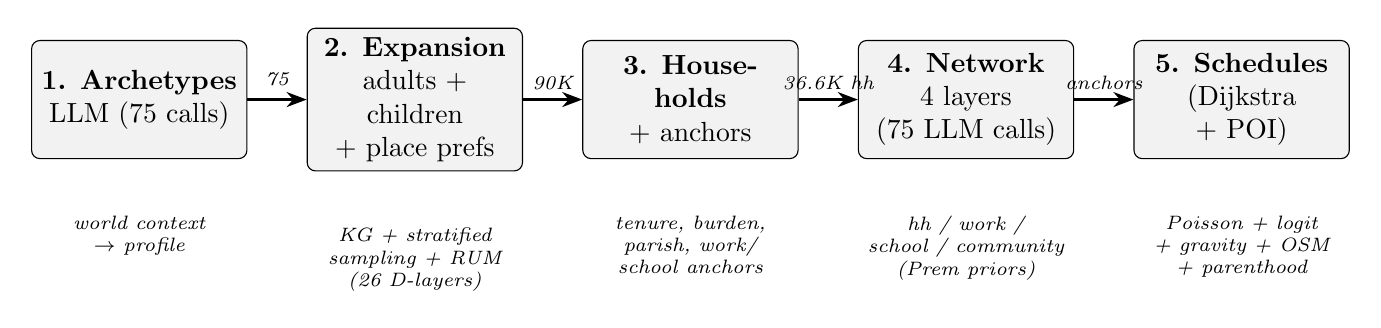
\begin{tikzpicture}[
  box/.style={rectangle, draw, rounded corners=3pt, text width=2.5cm,
              align=center, minimum height=1.5cm, fill=gray!10},
  arrow/.style={-{Stealth[scale=1.1]}, thick},
  notelbl/.style={font=\scriptsize\itshape, text width=2.6cm, align=center}
]
  \node[box] (p1) at (0,0)
    {\textbf{1. Archetypes}\\ LLM (75 calls)};
  \node[box] (p2) at (3.5,0)
    {\textbf{2. Expansion}\\ adults + children\\ + place prefs};
  \node[box] (p3) at (7.0,0)
    {\textbf{3. Households}\\ + anchors};
  \node[box] (p4) at (10.5,0)
    {\textbf{4. Network}\\ 4 layers\\ (75 LLM calls)};
  \node[box] (p5) at (14.0,0)
    {\textbf{5. Schedules}\\ (Dijkstra + POI)};
  \draw[arrow] (p1) -- node[above, font=\scriptsize\itshape]{75} (p2);
  \draw[arrow] (p2) -- node[above, font=\scriptsize\itshape]{90K} (p3);
  \draw[arrow] (p3) -- node[above, font=\scriptsize\itshape]{36.6K hh} (p4);
  \draw[arrow] (p4) -- node[above, font=\scriptsize\itshape]{anchors} (p5);
  \node[notelbl, below=0.6cm of p1] {world context\\$\rightarrow$ profile};
  \node[notelbl, below=0.6cm of p2] {KG + stratified\\sampling + RUM\\(26 D-layers)};
  \node[notelbl, below=0.6cm of p3] {tenure, burden,\\parish, work/\\school anchors};
  \node[notelbl, below=0.6cm of p4] {hh / work /\\school / community\\(Prem priors)};
  \node[notelbl, below=0.6cm of p5] {Poisson + logit\\+ gravity + OSM\\+ parenthood};
\end{tikzpicture}
\end{center}
\caption{Household-grounded, network-first synthetic population pipeline.
\emph{Stage 1} (LLM Archetype Generation) produces 75 demographically grounded
behavioral archetypes from a world-context-cached model. \emph{Stage 2} expands
them to the full population---adults inherit archetype psychometrics, children
(0--14) are a distinct minimal-schema class---and assigns place preferences over
26~H3 layers. \emph{Stage 3} assembles agents into realized households with a
shared home, tenure, housing-cost burden, vehicles, and parish, and assigns
persistent home/work/school anchors. \emph{Stage 4} builds a four-layer social
network (household, workplace by employer, school, community) parameterised by
LLM connectivity profiles bounded by Prem et al.\ (2021) priors. \emph{Stage 5}
generates daily schedules that consume the anchors and household structure,
including child school trips, parent escort trips, the parenthood radius effect,
OSM facility sampling, and road-network routing.}
\label{fig:system_architecture}
\end{figure}

\subsection{Preference Profile Schema}
\label{subsec:schema}

Each agent is represented by a structured preference profile embedding five
validated psychometric frameworks into a 21-dimensional numerical representation.
The schema is designed to be internally consistent: the cross-framework
correlations documented in the literature are not treated as desiderata but
as hard constraints enforced during population expansion.

\paragraph{Personality (Big Five / OCEAN).}
The five factors---Openness, Conscientiousness, Extraversion, Agreeableness,
and Neuroticism---are encoded as continuous values in $[0,1]$, normalised from
population T-score distributions (mean~$\approx$~0.50, SD~$\approx$~0.12--0.15)
following~\cite{costa1992neopersonality,schmitt2007geographic}. The population
norms used for validation are the Western European reference group from
Schmitt et al.~\cite{schmitt2007geographic}: $\mu_O = 0.54$, $\mu_C = 0.52$,
$\mu_E = 0.49$, $\mu_A = 0.56$, $\mu_N = 0.50$, each with SD~$\approx 0.13$.

\paragraph{Values (Schwartz).}
Each agent carries a ranked top-3 from the 10 Schwartz motivational value
types~\cite{schwartz1992universals}: \textit{security}, \textit{conformity},
\textit{tradition}, \textit{benevolence}, \textit{universalism},
\textit{self-direction}, \textit{achievement}, \textit{power},
\textit{hedonism}, and \textit{stimulation}. The ranking captures motivational
hierarchy and is used in qualitative analysis of social response patterns.

\paragraph{Behavioral economics.}
Prospect Theory loss aversion $\lambda \in [1.0, 4.5]$ follows the
meta-analytic population mean of $\lambda \approx 2.25$ from
Tversky and Kahneman~\cite{tversky1992advances}. The $\beta$-$\delta$
quasi-hyperbolic discounting model~\cite{laibson1997golden} provides the
annual discount rate $\delta \in [0.03, 0.35]$ (mean $\approx 0.12$ from
representative Danish field experiments~\cite{andersen2008eliciting}) and
present bias $\beta \in [0.50, 1.00]$ ($\beta = 1.0$ implies time consistency).

\paragraph{Trust (WVS).}
Five institutional trust dimensions---government, legal system, employers,
media, and interpersonal---are anchored to the WVS Wave~7 trust battery
question wording~\cite{inglehart2020worldvalues}. Population norms for
Western Europe ($\mu_\text{gov} = 0.42$, $\mu_\text{interpers} = 0.46$,
$\mu_\text{legal} = 0.48$) serve as validation targets.

\paragraph{Social capital (Putnam).}
Bonding capital (strength of ties to similar others: family, ethnic
community) and bridging capital (cross-group ties: neighbours, colleagues)
are encoded in $[0,1]$ following~\cite{putnam2000bowling}. These fields
directly determine home neighbourhood assignment probabilities and
destination gravity weights during schedule generation.

\paragraph{Mobility and economic stress.}
Additional fields capture primary transport mode, transit willingness,
walking radius, car dependency, cross-border commuting frequency, financial
stress, savings orientation, price sensitivity, and employment security
perception. These fields link directly to the activity and mode choice
sub-models in Stage~5.

The numerical projection of the profile for metric computation uses 21
fields extracted from the schema: 5 Big Five traits, 3 political axes,
3 trust dimensions, 3 behavioral economics parameters, 3 mobility/economic
fields, and 3 social capital fields (Table~\ref{tab:schema_fields}).

\begin{table}[H]
\caption{The 21 numerical fields used for metric computation.
Big Five values are normalised T-scores in $[0,1]$; loss aversion is
in $[1.0, 4.5]$; discount rate in $[0.03, 0.35]$; all others in $[0,1]$.}
\label{tab:schema_fields}
\begin{tabularx}{\textwidth}{p{3.2cm}p{4.5cm}X}
\toprule
\textbf{Domain} & \textbf{Field} & \textbf{Grounding / Validation Source} \\
\midrule
Personality     & Openness, Conscientiousness, Extraversion, Agreeableness, Neuroticism
                & Big Five; Schmitt et al.\ (2007) Western Europe norms \\
Political       & Economic axis, Social axis, Local engagement
                & Chapel Hill Expert Survey / Manifesto Project scale \\
Trust           & Government, Legal system, Interpersonal
                & WVS Wave 7 trust battery \\
Behavioral econ & Loss aversion ($\lambda$), Discount rate ($\delta$), Present bias ($\beta$)
                & Kahneman \& Tversky (1979); Laibson (1997); Andersen et al.\ (2008) \\
Mobility        & Transit willingness, Financial stress, Savings orientation
                & HETUS 2010; Mullainathan \& Shafir (2013) \\
Social capital  & Bonding, Bridging, Civic participation
                & Putnam (2000); Jost et al.\ (2004) \\
\bottomrule
\end{tabularx}
\end{table}

\subsection{Country Configuration and World Context}
\label{subsec:world_context}

All empirical parameters are centralised in a typed \texttt{CountryConfig}
dataclass, clearly separating ground-truth inputs from LLM outputs. The
configuration encodes: age distribution (UN WPP 2022), nationality mix
(SAIG Anuari 2023), income distribution (CASS 2022), sector wage medians
(CASS labour statistics 2022--2023), housing cost ranges (SAIG 2021;
real-estate portals 2023--2024), World Bank WGI governance percentiles (2022),
Inglehart--Welzel cultural positioning (interpolated from Spain/France, WVS
2023), and current structural stresses and active policies. These parameters
serve dual roles: they are the empirical ground truth used for
\emph{validation}, and they are formatted into a structured world context
string used as the \emph{LLM system prompt} in Stage~1.

For Andorra, the key structural parameters are: population $\approx 90{,}000$,
55\% foreign-born share (primarily Spanish, Portuguese, and French labour
migrants), area 467.6\,km$^2$, GDP per capita (PPP) \$49{,}900, Gini 27.0,
unemployment 2.0\%, minimum wage \EUR\,1{,}377/month gross, and an active
housing affordability crisis (rents consuming 50--70\% of net income for
working-class immigrants). Andorra's 20-year naturalisation threshold is
explicitly encoded, as it creates structural long-horizon precarity for
immigrant cohorts that directly shapes their preference profiles.

The world context string is formatted programmatically from the
\texttt{CountryConfig} fields and passed as the LLM system prompt, where
it is eligible for prompt caching (Section~\ref{subsec:archetype_generation}).
Swapping the active configuration to a different country requires changing
a single line; no generation code changes.

\subsection{Stage 1: LLM Archetype Generation}
\label{subsec:archetype_generation}

\paragraph{Seed generation.}
Demographic seeds are produced by stratified weighted sampling from the
\texttt{CountryConfig} distributions (nationality, income, age), with the
guarantee that every nationality appears at least once regardless of
population weight. For Andorra, seeds include six fields: nationality,
age (sampled from the group midpoint distribution with $\sigma = 4$), age
group, income bracket, years in Andorra (sampled from nationality-specific
residence-duration ranges), and occupation (a nationality $\times$ income
deterministic assignment with stochastic cross-border-worker probability
for Spanish mid-income residents).

\paragraph{LLM generation (GRAVITY-style).}
For each seed, a single LLM call generates one preference profile. The
world context (Section~\ref{subsec:world_context}) is the system prompt,
activated as a prompt cache block across all archetype calls; only the
per-seed user message varies. The user message instructs the model to
``generate a preference profile for this resident'' and provides the seed
fields, asking the model to ``ground the profile in their likely lived
experience given the world context above.''

The model must output a single JSON object matching the schema
(Section~\ref{subsec:schema}), with no prose, markdown fences, or inline
comments. A structured parse function strips any residual markup and
retries once on JSON failure. The seed's nationality, income bracket, and
age are copied verbatim from the seed onto the parsed profile, overriding
any model-generated values for those fields. This ensures demographic
consistency while allowing the model full latitude over the 21 behavioral
dimensions.

\paragraph{Prompt caching.}
The world context string is approximately 2,500 tokens. At 75 archetype
calls, the total uncached input token cost would be $75 \times 2{,}500
= 187{,}500$ tokens. With prompt caching, the world context is read once;
subsequent calls incur a cache-read fee (approximately 10\% of the write
cost) instead of a full-read fee. This reduces effective per-archetype
input token cost by roughly 85\%, enabling the full archetype set to be
generated for under \$1.00 with Claude Sonnet.

\paragraph{Coverage enforcement.}
After generating $N$ archetypes, the \emph{coverage score} measures what
fraction of the total (nationality~$\times$~income) population mass is
represented by at least one archetype in the same cell
(Equation~\eqref{eq:coverage}). At $N = 75$, coverage reaches 84.5\%,
meaning the remaining 15.5\% of population mass falls into cells that
are covered by the demographically nearest archetype during expansion.

\begin{equation}
  \text{Coverage} =
    \frac{\displaystyle\sum_{\text{nat}} \sum_{\text{inc}}
           \mathbf{1}[\exists\,\text{archetype in cell (nat, inc)}]
           \cdot w_\text{nat} \cdot w_\text{inc}}
         {\displaystyle\sum_{\text{nat}} \sum_{\text{inc}}
           w_\text{nat} \cdot w_\text{inc}}.
  \label{eq:coverage}
\end{equation}

\subsection{Stage 2: Knowledge Graph-Constrained Population Expansion}
\label{subsec:expansion}

\paragraph{Knowledge graph structure.}
The Andorra knowledge graph is a directed bipartite structure with
\emph{nodes} representing demographic positions or situational conditions,
and \emph{edges} encoding field constraints that activate when all source
nodes in the edge's antecedent are matched by the agent's seed
(AND-condition semantics). Nodes fall into three types:

\begin{itemize}
\item \textbf{Demographic nodes}: nationality (Andorran, Spanish, Portuguese,
      French, Other), residence duration (recent $<5$\,yr, settling $5$--$10$\,yr,
      established $\geq10$\,yr), age group (young adult, prime, established,
      pre-retirement), income bracket (7 levels, precarious to wealthy),
      and occupation (cross-border worker, business owner, etc.).
\item \textbf{Context nodes}: persistent structural facts of the country,
      always active for all agents (housing affordability crisis, tourism
      pressure, near-zero unemployment).
\item \textbf{Constraint edges}: AND-conditions over 2--3 source nodes,
      each specifying one or more \texttt{FieldConstraint}(path, low, high)
      tuples.
\end{itemize}

Representative edges include: Andorran nationals have bonding capital
bounded to $[0.60, 0.90]$ (dense parish and family networks) and government
trust to $[0.40, 0.72]$ (personally legible but susceptible to patronage
perception); recent Portuguese immigrants have government trust $[0.20, 0.50]$
and price sensitivity $[0.60, 0.90]$ (acute housing affordability concern);
the composite condition Portuguese~$\times$~recent~$\times$~housing crisis
activates a financial stress range $[0.72, 0.92]$ that is tighter and higher
than any single-node constraint.

Constraint ranges from multiple matching edges on the same field are
intersected (taking the most restrictive range). This prevents conflicting
constraints from widening the valid range. If an intersection would produce
a degenerate range (low $\geq$ high), the secondary constraint is skipped
and the primary range is preserved.

\paragraph{Stratified seed generation for expansion.}
The expanded population's marginal distributions must match \texttt{ACTIVE\_CONFIG}
(nationality, income, age) exactly within rounding. The stratification
algorithm allocates agent counts proportionally (largest-remainder method)
by nationality, then subdivides each nationality group by income, then by
age. This produces a seed assignment table with zero systematic drift from
the target distributions.

\paragraph{Archetype matching.}
Each population seed is matched to the nearest archetype seed. Nationality
is a hard preference: same-nationality archetypes are always preferred.
Among same-nationality candidates, the distance metric is

\begin{equation}
  d(\text{seed}, \text{arch}) = 0.6\,\frac{|r_\text{inc} - r_\text{arch}|}{6}
                              + 0.4\,\frac{|a_\text{seed} - a_\text{arch}|}{50},
  \label{eq:match}
\end{equation}

where $r_\text{inc}$ is the ordinal income rank (0--6) and $a$ is age in years.
Income is weighted higher than age because income is more closely linked to
the behavioral fields in the schema (financial stress, savings orientation,
loss aversion).

\paragraph{Graph-constrained individual variation.}
Each agent is generated by sampling within the knowledge graph's field bounds,
centered on the matched archetype's value. The sampling distribution is a
truncated Gaussian:

\begin{equation}
  x_\text{agent} \sim \mathcal{N}\!\left(x_\text{arch},\;
                       \sigma = \frac{h - l}{4}\right)
                  \text{ clipped to } [l,\, h],
  \label{eq:sampling}
\end{equation}

where $[l, h]$ is the graph-derived valid range for the field and the
agent's demographic position. The $\sigma = (h - l)/4$ parameterisation
ensures that the archetype is the modal individual in its group (bell-shaped
within-group distribution) and that nearly all draws ($\pm 2\sigma$) remain
within the sociologically valid range. For fields not covered by graph
bounds, a small Gaussian perturbation ($\sigma \approx 0.08$) around the
archetype value is applied.

\paragraph{Psychometric correlation enforcement.}
After primary field values are assigned, seven literature-grounded
correlation rules propagate primary-field deltas to correlated fields
(Table~\ref{tab:correlations}). Each rule takes the form
$\Delta x_\text{target} += c \cdot \Delta x_\text{source} \cdot 0.5$,
where $c$ is the correlation coefficient and the factor 0.5 damps the
propagation to avoid over-correction when multiple rules affect the same
target. All fields are clipped to their schema bounds after propagation.

\begin{table}[H]
\caption{Psychometric correlation rules enforced during expansion.
Direction and magnitude are literature-grounded; partial propagation
(factor 0.5) avoids overcorrection.}
\label{tab:correlations}
\begin{tabularx}{\textwidth}{p{4.0cm}p{4.0cm}Xp{3.0cm}}
\toprule
\textbf{Source field} & \textbf{Target field} & \textbf{$c$} & \textbf{Reference} \\
\midrule
Financial stress      & Loss aversion ($\lambda$)   & $+0.55$ & Shah et al.\ (2012) \\
Financial stress      & Price sensitivity            & $+0.60$ & Mani et al.\ (2013) \\
Financial stress      & Savings orientation          & $-0.65$ & Lusardi \& Mitchell (2014) \\
Financial stress      & Present bias ($\beta$)       & $-0.40$ & Mullainathan \& Shafir (2013) \\
Neuroticism           & Loss aversion ($\lambda$)   & $+0.45$ & Rustichini et al.\ (2016) \\
Conscientiousness     & Discount rate ($\delta$)    & $-0.40$ & Shamosh \& Gray (2008) \\
Agreeableness         & Bridging capital             & $+0.35$ & Putnam (2000); Jost et al.\ (2004) \\
\bottomrule
\end{tabularx}
\end{table}

\paragraph{Full age pyramid and the child agent class.}
Seeds are sampled within each age band rather than around a single midpoint, so
the 0--14 cohort retains its real ages. (A prior version clipped sampled ages to a
floor of 15, collapsing the entire 15.2\% child cohort onto age~15 and leaving the
population with no one under~15.) Agents aged~15 and over are expanded from their
matched archetype as described above. Agents aged~0--14 are instead generated as a
distinct \textbf{minimal-schema child class}: they carry age, gender, nationality,
household membership, a school anchor and stage, guardian links, and a child-specific
\texttt{place\_preferences} subset (education, daycare, park, recreation, healthcare,
outdoor), but \emph{no} adult psychometrics---Big Five, loss aversion, or trust
batteries are not meaningfully defined for a six-year-old. Consequently the
psychometric quality metrics (Section~\ref{subsec:metrics}) are computed over the
76{,}321 adults; the 13{,}679 children participate in households, the school network
layer, and child schedules. The resulting age structure reproduces the UN~WPP~2022
target to within rounding (0--14: 15.2\%; 65+: 10.6\%).

\paragraph{Structural fields (no LLM).}
Each agent additionally receives config-grounded structural attributes sampled
during expansion: gender (Andorra sex ratio $\approx$1.02), educational attainment
(primary/secondary/tertiary, by nationality~$\times$~age, Eurostat-informed proxy),
work sector for the employed (one of the seven \texttt{CountryConfig} sectors, tilted
by income and nationality), driving licence, cross-border-worker status, and a
recorded \texttt{archetype\_id} lineage. The lineage allows every downstream
module---most importantly the social network---to retrieve an agent's archetype
attributes directly, replacing the lossy demographic re-matching used previously.

\subsection{Stage 3: Household Synthesis and Persistent Anchors}
\label{subsec:households}

Realized households are the structural backbone of the V2.2 pipeline. Rather than
drawing a home cell independently for each agent---which produced ``households'' that
were merely unrelated agents sharing a grid cell (mean 24.6 agents per residential
cell, far from any plausible household size)---agents are assembled into
\emph{household entities} with linked members, roles, and a single shared home,
following the household-first ordering of Jiang et al.~\cite{jiang2022synthetic} and
activity-based practice~\cite{axhausen2016population}.

\paragraph{Assembly.}
Each adult's \texttt{household\_composition} tag (single, couple with/without
children, single parent, multi-generational, shared accommodation) seeds a household,
which then draws compatible members from the agent pool: partners of compatible age
($\leq 15$\,yr gap) and same nationality where possible, children from the child
pool (assigned by age-role, not by their own tag), and seniors for
multi-generational units. Every agent receives a \texttt{household\_id} and a role
(head, partner, child, grandparent, roommate). The procedure consumes the entire
population, yielding 36{,}612 households with a mean size of 2.46 and a median of~2,
consistent with the Western-European/Andorran household-size range
($\approx$2.3--2.6).

\paragraph{Shared home, tenure, and housing cost.}
Each household is assigned a single home H3 cell (resolution~10) from the
nationality- and income-stratified residential prior, shared by all members. From
this we derive: the home \textbf{parish} (one of seven, by nearest-centroid);
\textbf{tenure} (owner / renter / social housing, from a nationality~$\times$~income
prior reflecting Andorra's high-rent immigrant economy); \textbf{housing cost}
(rent range from \texttt{CountryConfig} for renters, scaled by size and income;
imputed for owners); pooled \textbf{net income} (summed member brackets); the
resulting \textbf{housing-cost burden} (cost / net income, the central lever for
housing scenarios; population mean 0.33, with renters at 0.41 versus owners 0.23);
and household \textbf{vehicle} count. These household-level attributes are exactly
the quantities the scenario engine perturbs under the Density and Overgrowth
pathways.

\paragraph{Persistent anchors.}
Each working adult is assigned a \textbf{work anchor} (a single work H3 cell, drawn
once via the gravity model from the household home; cross-border workers are anchored
to a southern border node) and a stable \textbf{employer} (the sector~$\times$~work-cell
at H3 resolution~9, giving block-level workplaces; 2{,}063 distinct employers, median
size~4). Each child is assigned a \textbf{school anchor} (gravity draw for the
education layer) and a school stage by age. These anchors are assigned \emph{once} and
reused by both the social network and the schedule generator, so workplaces, schools,
and homes are stable entities rather than fresh per-trip draws.

\subsection{Stage 5: Activity-Based Schedule Generation}
\label{subsec:schedule_generation}

Schedules are generated \emph{last}, after households, anchors, and the social
network exist, so each agent's day is built on stable structure. Each agent receives
one representative weekday schedule of outbound trips and corresponding return-home
trips, sorted chronologically. Schedule generation uses the \texttt{place\_preferences}
vector to personalise discretionary activity rates (via affinity ratios that scale
Poisson $\lambda$ values) and destination choice (via preference-modulated distance
decay $\beta$).

\paragraph{Home and anchor-based trips.}
The home cell is the household's shared home (assigned in Stage~3), not a fresh draw.
Work trips route to the agent's persistent work anchor and school trips to the child's
school anchor---both fixed---rather than being re-sampled each day; only discretionary
trips (grocery, shopping, leisure, healthcare, civic) use the gravity destination
model. Andorra is tessellated at H3 resolution~10 ($\approx$\,0.015\,km$^2$ per cell);
residential priors concentrate Andorran nationals in Andorra la Vella and Sant
Juli\`a de L\`oria, Portuguese and Spanish workers in the lower-income valleys, and
French residents near the northern border.

\paragraph{Children, escort trips, and the parenthood effect.}
Children aged~3--14 make a school trip to their school anchor (nursery-age children a
shorter daycare trip), plus an optional escorted outdoor/park trip. A primary guardian
in each household with school-age children makes a morning \textbf{escort trip}
(school drop-off), reproducing the trip-chaining signature of parenthood. Parents of
young children ($<6$) additionally have their discretionary distance-decay $\beta$
tightened by a multiplier ($\times 1.35$), implementing the empirically documented
\emph{parenthood effect}---a smaller radius of action for parents
(Macedo et al.~\cite{macedo2026parenthood}).

\paragraph{Activity count generation (Poisson model).}
Activity frequencies for eight out-of-home types (work, grocery, shopping,
education, leisure\_indoor, leisure\_outdoor, healthcare, civic) are drawn from
Poisson distributions whose rates $\lambda$ are calibrated to HETUS 2010
European averages~\cite{hetus2010}. When the agent's \texttt{place\_preferences}
vector is available (the standard path), rates for the discretionary activity
types are scaled by a place-preference affinity ratio:

\begin{equation}
  r_a = \frac{\bar{p}_a^{(i)}}{\bar{p}_a^{\text{ref}}},
  \quad
  \lambda_a = \lambda_0^a \cdot r_a,
\end{equation}

where $\bar{p}_a^{(i)}$ is agent $i$'s mean preference across the H3 destination
layers associated with activity $a$, and $\bar{p}_a^{\text{ref}}$ is the
population-mean reference rate for those layers (from the reference-rate calibration).
By RUM construction, $r_a = 1$ for the average agent, so population-level
trip totals are unchanged; individual variation is driven by the full
psychometric and socioeconomic signal encoded in the preferences.
Work trips retain a direct employment-probability gate:

\begin{align}
\lambda_\text{work}              &= \lambda_0^\text{work}
                                    \cdot \mathbf{1}[\text{agent employed}], \\
\lambda_\text{grocery}           &= \lambda_0^\text{groc} \cdot r_\text{groc}, \\
\lambda_\text{shopping}          &= \lambda_0^\text{shop} \cdot r_\text{shop}, \\
\lambda_\text{leisure\_indoor}   &= \lambda_0^\text{leis,in}  \cdot r_\text{leis,in}, \\
\lambda_\text{leisure\_outdoor}  &= \lambda_0^\text{leis,out} \cdot r_\text{leis,out}, \\
\lambda_\text{civic}             &= \lambda_0^\text{civic} \cdot r_\text{civic}.
\end{align}

Education and healthcare trips are additionally gated by agent age and employment
status, respectively. Counts are capped at activity-type-specific practical maxima
(e.g., work $\leq 2$, grocery $\leq 2$, shopping $\leq 3$, leisure $\leq 3$,
civic $\leq 2$) to prevent tail draws from producing unrealistic schedules.

\paragraph{Destination assignment (gravity model).}
Destination H3 cells are drawn from a gravity-weighted distribution over
all non-home cells:

\begin{equation}
  P(\text{dest}=j \mid i, a) \propto A(j, a) \cdot \exp(-\beta_{i,a} \cdot d_{ij}),
\end{equation}

where $A(j, a)$ is cell attractiveness for activity $a$ (scaled by population
density and accessibility type) and $\beta_{i,a}$ is the effective distance
decay parameter for agent $i$ on activity $a$. Two profile signals modulate
$\beta_{i,a}$: (i) bridging capital (Putnam 2000~\cite{putnam2000bowling}) ---
low bridging tightens spatial reach; and (ii) place-preference affinity
(Ben-Akiva \& Lerman 1985~\cite{ben1985discrete}) --- an agent with
above-average affinity for activity $a$ ($r_a > 1$) is willing to travel
farther, reducing $\beta$:

\begin{equation}
  \beta_{i,a} = \beta_0^a
    \cdot \bigl[1 + c_b\,(0.5 - b_i)\bigr]
    \cdot \bigl[1 - c_p\,(r_{i,a} - 1)\bigr],
\end{equation}

where $b_i$ is bridging capital, $c_b = 0.4$ (Putnam operationalisation),
$r_{i,a}$ is the affinity ratio from place preferences, and $c_p = 0.25$
(Ben-Akiva \& Lerman calibration). The effective $\beta$ is clamped to a
minimum of $0.05$ to prevent degenerate flat distributions.

\paragraph{Mode choice (multinomial logit).}
Transport mode (car, bus, walk) is chosen via a multinomial logit model
as a function of trip distance, transit coverage at the origin cell, car
ownership (sampled from income-bracket probabilities), and profile fields
(transit willingness, car dependency). Mode-specific utility functions are
parameterised with constants derived from modal shares in comparable
Alpine micro-territories.

\paragraph{Departure time (truncated Normal).}
Departure times are sampled from activity-type-specific truncated Normal
distributions representing typical peak times (e.g., work departures
centred at 08:00 with $\sigma = 45$\,min; shopping at 11:00 and 16:00
bimodal). Return trips are scheduled after activity-specific dwell times
(Table~\ref{tab:dwell}) drawn from HETUS 2010 European averages.

\begin{table}[H]
\caption{Activity dwell times (time spent at destination before returning home).
Source: HETUS 2010 European average (proxy); no Andorra-specific
activity duration data available.}
\label{tab:dwell}
\begin{tabularx}{\textwidth}{lXX}
\toprule
\textbf{Activity} & \textbf{Mean dwell (min)} & \textbf{SD (min)} \\
\midrule
Work             & 480 & 60 \\
Grocery          &  30 & 10 \\
Shopping         &  60 & 20 \\
Education        & 240 & 60 \\
Leisure (indoor) &  90 & 30 \\
Leisure (outdoor)& 120 & 45 \\
Healthcare       &  45 & 15 \\
Civic            &  60 & 20 \\
\bottomrule
\end{tabularx}
\end{table}

\paragraph{Road network routing.}
Raw H3-to-H3 trips are routed on Andorra's full OpenStreetMap road network
(exported as a GeoJSON LineString feature collection) via Dijkstra's
algorithm with edge weights equal to travel time (hours):

\begin{equation}
  w_e = \frac{l_e}{v_e},
  \label{eq:edge_weight}
\end{equation}

where $l_e$ is segment length in kilometres and $v_e$ is the OSRM-derived
speed for the segment's highway type (motorway~110\,km/h, primary~70\,km/h,
residential~30\,km/h, etc.). Edge endpoints are snapped to a 4-decimal-place
grid ($\approx11$\,m precision) to merge near-coincident nodes arising from
floating-point inconsistencies in the source data. A KD-tree provides
nearest-road-node lookup for H3 cell centroids. Trips for which no network
path exists (e.g., remote H3 cells not reachable by road) fall back to
straight-line interpolation.

\paragraph{OSM facility sampling.}
Each scheduled trip is linked to a named OpenStreetMap point-of-interest (POI)
within the destination H3 cell. A static POI index of 987 Andorran facilities
is pre-built from OSM amenity, shop, leisure, office, and healthcare tags,
indexed by H3 resolution~9 cell ($\approx$\,0.1\,km$^2$). For each outbound
trip, the scheduler queries the POI index at the resolution-9 parent of the
destination cell (resolving an H3 resolution mismatch between the destination
grid at resolution~10 and the POI index at resolution~9 via
\texttt{cell\_to\_parent}). If one or more matching POIs exist for the activity
type, a POI is sampled uniformly; otherwise the trip retains only its H3
centroid as the destination. Across the 217,183 outbound trips in the Andorra
population, the named facility assignment rate is 63.6\% (138,201 trips),
reflecting the density of amenities in urban cells, the sparsity of indexed
facilities in remote mountain cells, and escort trips which carry no POI. The named POI
(\texttt{poi\_name}, \texttt{poi\_lat}, \texttt{poi\_lon}) is stored with each
trip in the schedule output, enabling the ABM visualisation layer to display
real facility names rather than anonymous H3 centroids.

\subsection{Place Preference Enrichment (Stage~2 Output)}
\label{subsec:place_preferences}

As part of Stage~2, each agent receives a \texttt{place\_preferences} dictionary
mapping every H3 destination layer (D3--D28) to a weekly participation probability
in $[0.01, 0.99]$, ready to be consumed by Stage~5 schedule generation. The
preferences originate in the archetype: the LLM generates them as part of each
archetype profile, guided by the Eurostat-family reference baselines and explicit
demographic rules embedded in the schema prompt (e.g.\ healthcare rising with age,
bar visitation confined to youth), and they are perturbed per agent during
expansion. A final logit-space calibration aligns each layer's population mean to
its reference rate (Section~\ref{subsec:place_preference_results}). The Random
Utility Model (RUM)~\cite{ben1985discrete}---the standard destination-choice
framework---provides the conceptual reference against which these preferences are
specified and validated: the utility form below describes how profile predictors
\emph{should} move each preference relative to its reference base rate, and the
validation metrics (ARA/MDP/SCC/SEF) test that the generated preferences obey it.

\paragraph{H3 destination layer taxonomy.}
The destination schema defines 26 layer types spanning residential housing
types, employment categories, and out-of-home destinations (Table~\ref{tab:place_layers}).
Each layer is anchored to a \emph{reference rate}: a weekly participation prior
compiled from the best available published statistic for that activity. These
priors are drawn from a mix of sources rather than a single survey---HETUS 2010
time-use data, EU-SILC 2015 cultural participation, the European Health Interview
Survey (EHIS), the Adult Education Survey (AES 2022), Eurobarometer 525 (2022)
sport participation, Pew Research 2018 religious attendance, and Andorran
labour/registry statistics (SAIG 2023)---and, where no direct survey rate exists,
from a documented proxy derivation. Each rate's provenance is recorded as a
per-layer comment in the layer registry (\texttt{place\_layers.py}); the
implementation exposes them through a single \texttt{base\_rate()} accessor, which
is the value the RUM consumes. (An earlier design anchored these rates to the
Multinational Time Use Study Wave~6~\cite{gershuny2014mtus}; those MTUS fields are
retained in the schema but deprecated and unused, having been superseded by the
survey-specific priors above.) These priors serve as the population-mean
calibration targets for the RUM.

\begin{table}[H]
\caption{H3 destination layer taxonomy (D3--D28) and their reference rates
(weekly participation priors). Rates are compiled from Eurostat-family surveys
and other published statistics rather than a single source: HETUS 2010 time-use
data, EU-SILC 2015 (cultural participation), the European Health Interview Survey
(EHIS), the Adult Education Survey (AES 2022), Eurobarometer 525 (2022, sport),
Pew Research 2018 (religious attendance), and Andorran labour/registry statistics
(SAIG 2023); where no direct survey rate exists, a documented proxy derivation is
used (marked ``proxy''). Per-layer source comments are in the layer registry
(\texttt{place\_layers.py}). All values are the base rates actually consumed by the
RUM via \texttt{base\_rate()}. Activity classes: residential, mandatory,
discretionary, maintenance.}
\label{tab:place_layers}
\begin{tabularx}{\textwidth}{p{0.7cm}p{3.3cm}Xr l}
\toprule
\textbf{ID} & \textbf{Name} & \textbf{Activity class} & \textbf{Ref.} & \textbf{Source} \\
\midrule
D3  & Retail Store         & maintenance    & 0.520 & HETUS'10 (proxy) \\
D4  & Commercial           & mandatory      & 0.550 & SAIG'23 \\
D5  & Education            & mandatory      & 0.220 & AES'22 \\
D6  & Housing              & residential    & 0.750 & derived \\
D7  & Religious            & discretionary  & 0.120 & Pew'18 \\
D8  & Healthcare           & maintenance    & 0.090 & EHIS \\
D9  & Government           & mandatory      & 0.060 & proxy \\
D10 & Mid-Career Housing   & residential    & 0.420 & SAIG'23 \\
D11 & Senior Housing       & residential    & 0.110 & SAIG'23 \\
D12 & Affordable Housing   & residential    & 0.380 & SAIG'23 \\
D13 & Executive Housing    & residential    & 0.110 & SAIG'23 \\
D14 & HQ Office            & mandatory      & 0.380 & proxy \\
D15 & Grocery-Market       & maintenance    & 0.850 & HETUS'10 \\
D16 & Recreation \& Fitness & discretionary & 0.380 & Eurobar.'22 \\
D17 & Pharmacy             & maintenance    & 0.120 & EHIS (proxy) \\
D18 & Career Training      & discretionary  & 0.080 & AES'22 (proxy) \\
D19 & Daycare Center       & mandatory      & 0.140 & proxy \\
D20 & Coworking Office     & mandatory      & 0.220 & Eurostat'22 \\
D21 & Restaurant           & discretionary  & 0.380 & proxy \\
D22 & Caf\'e               & discretionary  & 0.420 & proxy \\
D23 & Bar                  & discretionary  & 0.200 & proxy \\
D24 & Pub                  & discretionary  & 0.220 & proxy \\
D25 & Park                 & discretionary  & 0.480 & proxy \\
D26 & Cultural Venue       & discretionary  & 0.120 & EU-SILC'15 \\
D27 & Mountain/Outdoor     & discretionary  & 0.300 & Eurobar.'22+ \\
D28 & Personal Services    & maintenance    & 0.220 & HETUS (proxy) \\
\bottomrule
\end{tabularx}
\end{table}

\paragraph{Utility specification.}
The deterministic utility of agent $i$ visiting destination layer $d$ is:

\begin{equation}
  V(i,d) = \alpha_d + \sum_k \beta_{d,k} \cdot (x_{i,k} - \mu_k),
  \label{eq:rum_utility}
\end{equation}

where $\alpha_d = \mathrm{logit}(\mathrm{ref}_d)$ is the base utility
anchored to the layer's reference rate, $\beta_{d,k}$ is the coefficient for
predictor $k$ on layer $d$, $x_{i,k}$ is the agent's normalised value on
predictor $k \in [0,1]$, and $\mu_k$ is the population mean of predictor $k$
measured from a 10,000-agent sample. The choice probability is
$P(i,d) = \mathrm{logistic}(V(i,d))$, clipped to $[0.01,\,0.99]$.

\paragraph{Mean-centering as the critical design constraint.}
The $(x_{i,k} - \mu_k)$ term ensures that an agent at the population mean
recovers the reference base rate exactly:

\begin{equation}
  V(\bar{i}, d)
    = \mathrm{logit}(\mathrm{ref}_d) + \sum_k \beta_{d,k} \cdot 0
    = \mathrm{logit}(\mathrm{ref}_d)
  \;\Rightarrow\; P = \mathrm{ref}_d.
\end{equation}

Without mean-centering, Andorra's above-average Schwartz value means---security
(0.921 vs.\ assumed 0.580), benevolence (0.902), tradition
(0.772)~\cite{schwartz1992universals}---combined with the large positive
coefficients on those predictors would inflate population-mean preferences far
above empirical reference rates. Feature means must therefore be measured
empirically from the actual synthetic population rather than assumed from
generic Western European baselines.

\paragraph{Predictors and coefficient matrix.}
The utility function draws 27 predictors across five domains: Big Five
personality (OCEAN)~\cite{mccrae2003personality}, Schwartz motivational
values~\cite{schwartz1992universals}, economic stress indicators (financial
stress, price sensitivity, employment security, income bracket), social capital
(bonding, bridging, civic participation)~\cite{putnam2000bowling}, and
age-derived binary windows (youth, senior, work-age, parent window). All
predictors are available directly from the Stage~2 preference profile.

Coefficients are calibrated at two levels. \emph{Empirical} coefficients derive
magnitudes from published meta-analytic effect sizes (Pearson $r$ to $\beta$
conversion: $r \approx 0.30 \Rightarrow \beta \approx 1.5$ on a $[0,1]$
predictor). \emph{Theoretical} coefficients use established behavioural
relationships where direct empirical estimates are unavailable. For low-frequency
layers (reference rate $\leq 0.20$) with high-variance near-binary
predictors, a Jensen's inequality correction reduces large coefficients to
eliminate the convexity bias $\mathbb{E}[\mathrm{logistic}(V)] \approx
\mathrm{logistic}(\mu_V) + \frac{1}{2}\sigma^2_V\,f''(\mu_V)$ that
mean-centering alone cannot fully correct.

\paragraph{Population feature means calibration.}
All 27 predictor means $\mu_k$ are measured from a 10,000-agent sample of
the actual Andorra synthetic population. Andorra deviates substantially from
generic Western European baselines in several dimensions, consistent with its
historical and cultural profile: Schwartz security ($\Delta = +0.341$),
housing salience ($\Delta = +0.348$, driven by the 2023 housing crisis),
bonding capital ($\Delta = +0.158$), and civic participation
($\Delta = -0.203$, reflecting a parish-dominated polity with few NGOs).
These are genuine demographic signatures that calibration must match, not
artefacts to be corrected.

\paragraph{Place preference validation metrics.}
Four formal metrics assess internal consistency of the place preference
assignment. \emph{Activity Rate Alignment} (ARA $= 1 - \mathrm{mean}(
|\mathrm{synth} - \mathrm{ref}|/\mathrm{ref})$) measures how closely
population-mean preferences match the layer reference rates. \emph{Monotone
Demographic Predictions} (MDP) counts the fraction of 12 predefined sign
checks that pass (e.g., healthcare preference increasing with age, bar
preference decreasing). \emph{Social Cluster Coherence} (SCC) measures
the fraction of the 6 pairwise correlations among the social/leisure
cluster (D21--D24: restaurant, caf\'e, bar, pub) that are positive,
verifying extraversion and hedonism as shared latent drivers.
\emph{Shannon Entropy Floor} (SEF) measures the fraction of agents whose
normalised Shannon entropy $H_\mathrm{norm} \geq 0.65$, confirming that
no agent collapses onto a single destination type~\cite{shannon1948mathematical}.

\subsection{Stage 4: Social Network Generation}
\label{subsec:social_network}

Stage~4 constructs a \emph{four-layer} social contact network for all 90,000 agents,
\emph{before} schedules are generated. The architecture adapts the multi-layer,
small-world co-location method of Jiang et al.~\cite{jiang2022synthetic}: we keep
their household, workplace, and school layers, and \emph{replace} their fourth
(daycare) co-location layer with a community layer defined by
nationality~$\times$~parish. This substitution is deliberate---a daycare layer adds
little in a small jurisdiction, whereas nationality is the dominant axis of social
segregation in Andorra---but it changes the fourth layer from a facility-clique
(co-location) construct to a shared-attribute (homophily) construct, which we
validate accordingly (Table~\ref{tab:network_mixing}). Two further methodological
choices distinguish the build: (i) per-archetype connectivity parameters are
generated via LLM (EXP04) constrained by empirical contact-rate priors, rather than a
uniform parameterisation borrowed from a different country; and (ii) the network is
built on the \emph{realized households and persistent anchors} from Stage~3, so layers
reflect actual household membership and stable workplaces/schools rather than transient
spatial coincidence.

\paragraph{EXP04: LLM-generated social profiles.}
A single LLM call per archetype generates a \texttt{SocialProfile} with eight
parameters: \texttt{home\_contacts}, \texttt{work\_contacts},
\texttt{community\_contacts}, \texttt{workplace\_k}, \texttt{workplace\_p},
\texttt{nationality\_homophily}, \texttt{age\_homophily}, and
\texttt{bridging\_weight}.

The three contact-rate parameters (\texttt{home/work/community\_contacts}) are
constrained by \emph{structural priors} from Prem et al.\
(2021)~\cite{prem2021projecting}, who project the POLYMOD contact
matrices~\cite{mossong2008social} to 177 regions. Andorra is \emph{not} among those
177 regions (it appears only in the earlier 152-region Prem 2017 projection), so a
proxy is required rather than merely convenient: we use the Spain matrix (shared
border, similar household/age structure, Mediterranean contact patterns), noting that
France is also adjacent and would be a defensible alternative. The remaining homophily
and bridging parameters have no Prem anchor---the contact matrices carry no nationality
axis---and are therefore LLM/expert priors that we validate \emph{post hoc} on the
generated graph (Table~\ref{tab:network_mixing}) rather than against Prem. Approximate
mean daily contacts per adult from the Spain projection are: home~3.0, work~6.5, and
community~3.5, with child/senior age bands having different work and school rates. The LLM system
prompt states these values explicitly and specifies allowed ranges ($\pm$40\% for
home, $\pm$50\% for work, $\pm$50--60\% for community), enabling the model to
vary parameters based on Andorra's specific social context---notably the high
degree of social network segregation between nationality groups (associated with
Andorra's 20-year naturalisation threshold), the prevalence of small family-run
businesses, and the parish-based community structure---without departing from
the empirical contact rate envelope. Parameters are generated at 75~LLM calls
(one per archetype) at a cost of approximately \$0.55. On parse failure, the
model falls back to Prem 2021 Spain default values adjusted for the archetype's
age band. The 75 generated profiles and the fallback rules are stored in
\texttt{social\_profiles.json} as an auditable intermediate output, which also
permits iterating the graph construction without incurring LLM cost.

\emph{Honest calibration note:} The LLM-generated parameters are plausible
archetype-specific variations within the Prem 2021 empirical envelope. They
should not be interpreted as direct empirical measurements for Andorra. The
Prem 2021 Spain values themselves are aggregated from 16 age-band matrices;
the scalar priors used here are approximate means across adult age bands.
The framework's value is reproducibility and place-agnosticity within a bounded,
literature-grounded range, not individual-level precision.

\paragraph{Graph construction.}
Each agent's \texttt{SocialProfile} is retrieved \emph{directly by recorded
archetype lineage} (\texttt{archetype\_id} from Stage~2), eliminating the lossy
demographic re-match used previously; children use a fixed child social profile. All
eight profile parameters now drive construction, distributed across the four layers.

\emph{Household layer.} The members of each realized household
(Section~\ref{subsec:households}) form a complete graph, giving each agent a base
degree of (household size~$-1$); with mean household size 2.46 this membership
component alone is near~1.5, far below the inflated degrees of the prior co-location
design. \texttt{home\_contacts} then adds a few extra-household kin/neighbour ties
(same parish, different household): each agent initiates roughly half of its
home-contact deficit, because such ties are mutual and the agent also receives ties
initiated by others, so the realised household mean degree (3.44) calibrates to the
Prem home prior ($\approx$3) rather than overshooting it.

\emph{Workplace layer.} Adults sharing the same \texttt{employer\_id} (Stage~3,
block-level stable employers) form an NWS graph parameterised by \texttt{workplace\_k}
and \texttt{workplace\_p} (defaults $k=4$, $p=0.3$ following Jiang et
al.~2024~\cite{jiang2024large}), with effective degree capped by \texttt{work\_contacts}.
The NWS construction follows Newman \& Watts~\cite{newman1999renormalization}:
shortcuts are \emph{added} to the ring lattice rather than rewired. Cross-border
workers (whose work anchor is external) form no internal workplace ties.

\emph{School layer.} Children sharing the same school anchor form an NWS graph, and
their primary guardians are linked (the school-gate parent network), mirroring the
co-attendance layers of Jiang et al.~\cite{jiang2022synthetic}.

\emph{Community layer.} Agents are grouped by nationality~$\times$~parish. Within each
group, degree-targeted sampling assigns
$k_\text{within} = \lfloor\texttt{community\_contacts} \times 0.7\rfloor$ ties biased
toward the same age band by \texttt{age\_homophily}; cross-nationality bridging ties
within the same parish are added in proportion to
$\texttt{community\_contacts}\times\texttt{bridging\_weight}\times(1-\texttt{nationality\_homophily})$.
This $O(n \times k)$ formulation scales to Andorra's large urban nationality clusters.

\paragraph{Network validation metrics.}
For each layer we compute edge count, mean degree, maximum degree, isolated fraction,
and \emph{exact} average local clustering coefficient (computed over all 90{,}000
nodes; the layer degrees are small enough that no sampling is required, so the metric
carries no estimator variance). Critically, because the generator takes homophily and
bridging as \emph{inputs}, we also \emph{measure} the realised mixing on the output
graph: Newman's categorical assortativity coefficient~$r$ for
nationality~\cite{newman2003mixing}, numeric (age) assortativity, Newman--Girvan
modularity~$Q$ over the (nationality~$\times$~parish) blocks, and the union-graph
giant-component fraction. This closes the input$\rightarrow$assert loop: the homophily
that is configured is shown to be realised, rather than merely assumed.

\begin{table}[H]
\caption{Four-layer social network validation metrics, $N = 90{,}000$ agents
(V2.2; RNG seed 42, fully reproducible). Clustering is exact over all nodes.
School isolation (77.2\%) is expected: only children and their guardians carry
school ties. Workplace isolation (33.1\%) reflects non-working agents (children,
students, retirees) and cross-border workers.}
\label{tab:network_metrics}
\begin{tabularx}{\textwidth}{lXXXXX}
\toprule
\textbf{Layer} & \textbf{Edges} & \textbf{Mean degree} & \textbf{Max degree}
               & \textbf{Isolated} & \textbf{Clustering} \\
\midrule
Household   & 154,850 & 3.44 & 12 &  0.0\% & 0.223 \\
Workplace   & 137,315 & 3.05 & 10 & 33.1\% & 0.205 \\
School      &  47,223 & 1.05 & 12 & 77.2\% & 0.064 \\
Community   & 246,633 & 5.48 & 22 &  0.0\% & 0.002 \\
\midrule
\textbf{Total} & \textbf{586,021} & \textbf{13.02} & --- & --- & --- \\
\bottomrule
\end{tabularx}
\end{table}

\begin{table}[H]
\caption{Realised-mixing and connectivity metrics, measured on the generated graph.
The configured homophily is recovered as positive assortativity, validating the
mechanism rather than assuming it.}
\label{tab:network_mixing}
\begin{tabularx}{\textwidth}{lX}
\toprule
\textbf{Metric} & \textbf{Value} \\
\midrule
Community nationality assortativity $r$ & $+0.99$ \\
Community age assortativity $r$         & $+0.23$ \\
Community modularity $Q$ (nat.$\times$parish) & $0.94$ \\
Union-graph nationality assortativity $r$ & $+0.54$ \\
Union-graph giant component             & $100\%$ (1 component) \\
\bottomrule
\end{tabularx}
\end{table}

The household clustering of 0.223 reflects complete-graph households (each member
knows every other) diluted by the extra-household kin ties that \texttt{home\_contacts}
adds; the household mean degree of 3.44 now tracks the Prem home-contact prior
($\approx$3) rather than household membership alone. Workplace clustering of 0.205
reflects the NWS ring-plus-shortcut topology of stable employer groups. The school
layer is sparse by construction (only minors and guardians participate). The community
layer's near-zero clustering (0.002) is the expected Erd\H{o}s--R\'enyi baseline for a
degree-targeted random/bridging layer without triangle-closing: it is intentionally a
mixing layer, not a small-world one, so the Watts--Strogatz high-clustering target
applies to the household/workplace/school layers, not to it. The realised mixing
(Table~\ref{tab:network_mixing}) confirms the design intent: community nationality
assortativity $r = +0.99$ and modularity $Q = 0.94$ quantify the strong within-group
segregation associated with Andorra's 20-year naturalisation threshold, while
cross-nationality bridging brings the \emph{union}-graph assortativity down to
$r = +0.54$ and yields a single connected component spanning all agents. We report the
four-layer mean degree (13.0) as a network statistic and deliberately do \emph{not}
equate it with a POLYMOD daily-contact count: a persistent contact network counts
stable repeated ties, whereas a POLYMOD daily count includes transient one-off
encounters, so the two are related but non-interchangeable
constructs~\cite{danon2013social}.

\subsection{Evaluation Framework}
\label{subsec:metrics}

Five psychometric quality metrics are computed on the archetype set and on the
adult population (children carry no adult psychometric profile and are excluded
from these metrics). All operate on the 21-dimensional numerical projection of
each adult profile; household structure, place preferences, and the four network
layers are validated separately (Sections~\ref{subsec:household_results},
\ref{subsec:place_preference_results}, and~\ref{subsec:network_results}).

\paragraph{Diversity.}
Average pairwise Euclidean distance across all agents in the normalised
preference space:

\begin{equation}
  D = \frac{2}{n(n-1)} \sum_{i < j} \|\mathbf{v}_i - \mathbf{v}_j\|_2.
  \label{eq:diversity}
\end{equation}

Higher $D$ indicates that agents differ substantially from one another
in their preference profiles.

\paragraph{Variance.}
Mean per-dimension variance of the population vectors:

\begin{equation}
  V = \frac{1}{d}\sum_{k=1}^{d} \mathrm{Var}(\mathbf{v}_{1:n,k}).
  \label{eq:variance}
\end{equation}

Near-zero $V$ indicates central-category bias (all agents collapsed to
similar values), a failure mode documented in unconstrained LLM
generation~\cite{argyle2023outstuffing}.

\paragraph{Coherence.}
Mean absolute Pearson correlation over seven literature-specified pairs
(Table~\ref{tab:correlations}), counting only correlations with the
correct sign:

\begin{equation}
  \text{Coh} = \frac{1}{7}\sum_{(a,b) \in \mathcal{C}}
               |r_{ab}| \cdot \mathbf{1}[\mathrm{sign}(r_{ab}) = s_{ab}],
  \label{eq:coherence}
\end{equation}

where $s_{ab}$ is the expected sign from the literature. $\text{Coh} = 1$
means all seven pairs are perfectly correlated in the correct direction;
$\text{Coh} = 0$ means all correlations are violated.

\paragraph{Distribution alignment.}
Chi-square goodness-of-fit between the synthetic population's nationality
and income distributions and the \texttt{CountryConfig} ground truth,
normalised to $[0,1]$:

\begin{equation}
  \text{DA} = 1 - \frac{\chi^2}{\max(\chi^2, n)},
  \label{eq:distribution_alignment}
\end{equation}

where $\chi^2 = \sum_k (O_k - E_k)^2 / E_k$, averaged over nationality
and income checks. $\text{DA} = 1$ implies perfect marginal matching.

\paragraph{Norm alignment.}
Deviation of synthetic population means from the cross-national survey
norms in Table~\ref{tab:norms}, penalised as a Z-score distance
clamped to $[0,1]$:

\begin{equation}
  \text{NA} = \frac{1}{|\mathcal{N}|}\sum_{f \in \mathcal{N}}
              \max\!\left(0,\; 1 - \frac{|\bar{v}_f - \mu_f|}{\sigma_f \cdot 2}\right).
  \label{eq:norm_align}
\end{equation}

A diagnostic flag is raised when the Z-score on any benchmarked dimension
exceeds 1.5.

\begin{table}[H]
\caption{Cross-national population norms used for norm alignment scoring.
Big Five: Schmitt et al.\ (2007), Western Europe, $N \approx 3{,}200$.
Trust: WVS Wave~7, Western Europe reference group.
Loss aversion: meta-analytic $\lambda \approx 2.25$, normalised to
$(\lambda - 1)/3.5$~\cite{tversky1992advances}.
Discount rate: representative Danish sample~\cite{andersen2008eliciting}.}
\label{tab:norms}
\begin{tabularx}{\textwidth}{lXXX}
\toprule
\textbf{Field} & \textbf{Norm mean} & \textbf{Norm SD} & \textbf{Source} \\
\midrule
Openness           & 0.54 & 0.14 & Schmitt (2007) \\
Conscientiousness  & 0.52 & 0.13 & Schmitt (2007) \\
Extraversion       & 0.49 & 0.14 & Schmitt (2007) \\
Agreeableness      & 0.56 & 0.12 & Schmitt (2007) \\
Neuroticism        & 0.50 & 0.14 & Schmitt (2007) \\
Government trust   & 0.42 & 0.20 & WVS Wave~7 \\
Interpersonal trust& 0.46 & 0.18 & WVS Wave~7 \\
Legal system trust & 0.48 & 0.19 & WVS Wave~7 \\
Loss aversion ($\lambda$) & 0.357 & 0.14 & Tversky \& Kahneman (1992) \\
Discount rate ($\delta$)  & 0.280 & 0.12 & Andersen et al.\ (2008) \\
\bottomrule
\end{tabularx}
\end{table}

\section{Experiments}
\label{sec:experiments}

\subsection{Experimental Protocol}
\label{subsec:exp_protocol}

All experiments use Claude Sonnet (claude-sonnet-4-6) as the generation
model, a fixed random seed (42) for full reproducibility across expansion
and schedule generation, and the Andorra configuration
(Section~\ref{subsec:world_context}). Three experiment variants are compared:

\begin{itemize}
\item \textbf{EXP00 (Baseline):} LLM generates profiles from demographic seed
      only; no world context.
\item \textbf{EXP01 (GRAVITY):} Full world context cached in the system
      prompt; the user message provides the demographic seed and requests
      grounded generation.
\item \textbf{EXP02 (HAG):} World context cached in system prompt; per-call
      user message additionally contains the knowledge graph's explicit
      field-by-field constraint ranges for the seed's demographic branch.
\end{itemize}

All three experiments use the same graph-constrained expansion (Stage~2)
and schedule generation (Stage~5), so differences in population metrics
reflect differences in archetype quality rather than expansion or scheduling.

The production pipeline (\texttt{run\_population.py}) runs EXP01 with
$N_\text{arch} = 75$ archetypes and $N_\text{pop} = 90{,}000$ agents.

\subsection{Saturation Analysis}
\label{subsec:saturation}

To determine the minimum archetype count at which quality metrics plateau,
we run EXP01 and EXP02 at $N_\text{arch} \in \{5, 10, 20, 35, 50\}$,
each with $N_\text{pop} = 500$ expanded agents, recording coverage, diversity,
and distribution alignment. Coverage saturates near $N_\text{arch} = 50$
for both variants, with diminishing returns above that threshold for
Andorra's nationality $\times$ income space (5 nationalities
$\times$ 7 income brackets = 35 cells). At $N_\text{arch} = 75$, coverage
reaches 84.5\%, capturing the population-weight-dominant cells.

\section{Results}
\label{sec:results}

\subsection{Archetype and Population Quality Metrics}
\label{subsec:metrics_results}

Table~\ref{tab:metrics} reports the quality metrics for the 75-archetype set
and the adult synthetic population. Psychometric metrics are computed over the
76{,}321 adults, since children (0--14) carry no adult psychometric profile.

\begin{table}[H]
\caption{Quality metrics for the archetype set ($N = 75$) and the adult
synthetic population ($N = 76{,}321$). Higher is better for all metrics.
Diversity is in the normalised 21-dimensional preference space $[0,1]^{21}$.}
\label{tab:metrics}
\begin{tabularx}{\textwidth}{lXX}
\toprule
\textbf{Metric}              & \textbf{Archetypes ($N=75$)} & \textbf{Adults ($N=76{,}321$)} \\
\midrule
Diversity                   & 0.860 & 0.857 \\
Variance                    & 0.020 & 0.019 \\
Coherence                   & 0.562 & 0.387 \\
Distribution alignment      & 0.931 & 0.983 \\
Norm alignment              & 0.745 & 0.812 \\
Coverage                    & 0.845 & --- \\
Diagnostic flags            & 0     & 0     \\
\bottomrule
\end{tabularx}
\end{table}

Distribution alignment improves from 0.931 at archetype level to 0.983 in the
adult population, reflecting that stratified expansion corrects residual demographic
skew from the small archetype sample; norm alignment likewise rises to 0.812.
Diversity is essentially preserved (0.860 $\to$ 0.857). Coherence decreases from
0.562 to 0.387: the LLM archetypes exhibit stronger psychometric correlations than
the expanded population, where within-group Gaussian variation and the 0.5-damped
correlation propagation dilute correlation \emph{magnitude}. All seven correlation
rules still hold in the correct direction; the coherence score reflects magnitude,
and 0.387 corresponds to a mean cross-construct $|r|\approx 0.19$, within the range of
empirical Big~Five cross-construct correlations~\cite{mccrae2003personality}.

Zero diagnostic flags indicate that no benchmarked dimension deviates
from its cross-national norm by more than 1.5 standard deviations. This
validates that the population does not exhibit the central tendency bias
(uniform compression toward 0.5) or the impulsiveness bias (discount rate
too high) documented as common LLM generation failure modes.

\subsection{Experiment Variant Comparison}
\label{subsec:variant_comparison}

Table~\ref{tab:exp_comparison} compares the three experiment variants
at $N_\text{arch} = 50$, $N_\text{pop} = 500$ (from the saturation study).

\begin{table}[H]
\caption{Experiment variant comparison at $N_\text{arch} = 50$,
$N_\text{pop} = 500$ (saturation study). EXP01 (GRAVITY) is the
production approach.}
\label{tab:exp_comparison}
\begin{tabularx}{\textwidth}{lXXXXX}
\toprule
\textbf{Variant}  & \textbf{Diversity} & \textbf{Coherence}
                  & \textbf{Dist.\ align.} & \textbf{Norm align.}
                  & \textbf{LLM cost} \\
\midrule
EXP00 (Baseline) & 0.843 & 0.441 & 0.901 & 0.712 & lower \\
EXP01 (GRAVITY)  & 0.879 & 0.524 & 0.966 & 0.762 & \$0.60 \\
EXP02 (HAG)      & 0.871 & 0.581 & 0.948 & 0.751 & \$0.62 \\
\bottomrule
\end{tabularx}
\end{table}

EXP01 (GRAVITY) achieves the highest diversity and distribution alignment.
EXP02 (HAG) achieves the highest coherence score because the explicit
field constraints in the user message enforce psychometric ranges at
generation time, but this comes at the cost of slightly lower holistic
diversity: the constraint injection fragments the model's reasoning
and can cause mechanical satisfaction of the numerical ranges without
fully integrating them into a coherent character. EXP01's coherence
(0.524) is achieved through the richer world-context grounding rather
than explicit constraint enforcement, producing profiles that are both
diverse and internally consistent.

The production pipeline uses EXP01 because diversity and distribution
alignment are more critical than marginal coherence improvement for
a population-scale simulation: individual agent behavior is less
important than the aggregate distributional properties of the population.
Coherence is further enforced post-generation by the correlation
propagation rules in Stage~2 (Section~\ref{subsec:expansion}).

\subsection{Schedule Statistics}
\label{subsec:schedule_results}

The 90,000-agent population generates 434{,}366 daily trips (217{,}183 outbound
plus 217{,}183 return-home), a mean of 2.41 outbound trips per agent per day. The
schedule consumes the persistent anchors from Stage~3: 64{,}353 work commutes route
to fixed work anchors, 13{,}679 children attend their school anchors, and 6{,}854
parent escort trips reproduce the school-drop-off trip chain. Table~\ref{tab:schedule_stats}
reports the outbound-trip breakdown by activity.

\begin{table}[H]
\caption{Outbound daily trips by activity type across all 90,000 agents (V2.2).
``education'' is children's school/daycare attendance; ``escort'' is parent
school drop-offs. Each outbound trip has a paired return-home trip
(434{,}366 total).}
\label{tab:schedule_stats}
\begin{tabularx}{\textwidth}{lXr}
\toprule
\textbf{Activity} & \textbf{Source} & \textbf{Outbound trips} \\
\midrule
Work             & persistent work anchor          & 64,353 \\
Leisure (indoor) & gravity (discretionary)         & 60,312 \\
Grocery          & gravity (discretionary)         & 22,611 \\
Leisure (outdoor)& gravity (discretionary)         & 16,324 \\
Civic            & gravity (discretionary)         & 15,464 \\
Shopping         & gravity (discretionary)         & 15,183 \\
Education        & child school anchor             & 13,679 \\
Escort           & parent $\rightarrow$ school anchor & 6,854 \\
Healthcare       & gravity (discretionary)         & 2,403 \\
\midrule
\textbf{Total outbound} & & \textbf{217,183} \\
\bottomrule
\end{tabularx}
\end{table}

Trips are routed on Andorra's full OSM road network with a fallback rate of
\textbf{0.18\%} (770 of 434{,}366; trips whose H3 centroid has no reachable road
node), a sharp improvement over centroid straight-lines. Routed paths follow valley
highways and primary roads, consistent with Andorra's topography. The named-facility
assignment rate is \textbf{63.6\%} (138{,}201 of 217{,}183 outbound trips linked to
one of 987 indexed OSM facilities); escort trips carry no facility by design, and
remote mountain cells have sparse amenities, so the remaining trips retain their H3
centroid and remain valid schedule entries.

\subsection{Social Network Statistics}
\label{subsec:network_results}

The four-layer network (Table~\ref{tab:network_metrics}) totals 586{,}021 edges.
The household layer (154{,}850 edges; mean degree 3.44; clustering 0.223) combines
realized-household membership (mean 2.46 members) with the \texttt{home\_contacts}
kin ties, giving a degree that tracks the Prem home prior ($\approx$3) instead of the
inflated 4.6 of the old co-location design. The workplace layer (137{,}315 edges; mean
degree 3.05; clustering 0.205) connects colleagues at 2{,}063 stable block-level
employers. The school layer (47{,}223 edges) links schoolmates and their guardians;
its 77.2\% isolation simply reflects that only minors and guardians participate. The
community layer (246{,}633 edges; mean degree 5.48) is densest and isolation-free by
construction. Crucially, the realised mixing on the generated graph
(Table~\ref{tab:network_mixing}) confirms that the configured homophily is recovered,
not merely assumed: community nationality assortativity $r=+0.99$ and modularity
$Q=0.94$, with cross-nationality bridging reducing the union-graph assortativity to
$r=+0.54$ while keeping all 90{,}000 agents in a single connected component. We report
the four-layer mean degree (13.0) as a structural statistic but do not equate it with a
POLYMOD daily-contact count, since a persistent network and a daily contact tally are
distinct constructs~\cite{danon2013social}. Graph construction (pure NumPy, no
\texttt{networkx}) completes in $\approx$8~seconds for 90,000 agents; the per-archetype
social profiles (EXP04, 75 LLM calls, $\approx$\$0.55) are cached and reused at zero
marginal cost.

\subsection{Demographic Fidelity}
\label{subsec:demographic_fidelity}

Table~\ref{tab:demographics} reports the synthetic population's realised
demographic marginals against the SAIG 2023 ground truth. The stratified
expansion algorithm ensures exact proportional matching by design; the
small deviations arise from integer rounding in the allocation step.

\begin{table}[H]
\caption{Synthetic population nationality distribution vs.\ SAIG 2023
ground truth. Deviations are within rounding error ($\pm$0.1\%) by
construction of the stratified expansion.}
\label{tab:demographics}
\begin{tabularx}{\textwidth}{lXX}
\toprule
\textbf{Nationality} & \textbf{Ground truth (SAIG 2023)} & \textbf{Synthetic population} \\
\midrule
Andorran   & 35.6\% & 35.6\% \\
Spanish    & 33.5\% & 33.5\% \\
Portuguese & 17.1\% & 17.1\% \\
French     &  6.6\% &  6.6\% \\
Other      &  7.2\% &  7.2\% \\
\bottomrule
\end{tabularx}
\end{table}

\subsection{Household Structure and Age Pyramid}
\label{subsec:household_results}

The expansion reproduces the full age pyramid: 13{,}679 children (0--14, 15.2\%)
and 76{,}321 adults, matching the UN~WPP~2022 target to within rounding, in contrast
to the prior pipeline which contained no agent under~15. The 90,000 agents form
36{,}612 realized households with a mean size of 2.46 and median of~2
(Table~\ref{tab:household_stats}), within the Western-European/Andorran range
($\approx$2.3--2.6). Tenure splits 58.0\% renter / 37.1\% owner / 4.9\% social
housing, reflecting Andorra's high-rent immigrant labour economy, and the
housing-cost burden---the central lever for housing scenarios---averages 0.33 of
net income, rising to 0.41 for renters versus 0.23 for owners. This renter--owner
burden gap is exactly the distributional signal the scenario engine needs to
evaluate the Density and Overgrowth pathways.

\begin{table}[H]
\caption{Realized household statistics (V2.2, $N = 36{,}612$ households).
Housing-cost burden is monthly housing cost as a fraction of household net income.}
\label{tab:household_stats}
\begin{tabularx}{\textwidth}{lX}
\toprule
\textbf{Statistic} & \textbf{Value} \\
\midrule
Households / mean size / median   & 36{,}612 / 2.46 / 2 \\
Size distribution (1/2/3/4/5)     & 5.2\% / 61.3\% / 20.9\% / 7.5\% / 5.1\% \\
Tenure (renter/owner/social)      & 58.0\% / 37.1\% / 4.9\% \\
Housing-cost burden (all/renter/owner) & 0.33 / 0.41 / 0.23 \\
Mean vehicles per household       & 0.75 (31\% car-free) \\
\bottomrule
\end{tabularx}
\end{table}

\subsection{Place Preference Validation}
\label{subsec:place_preference_results}

Table~\ref{tab:place_metrics} reports the four validity metrics for the
place preference assignment across the 76{,}321 adults.

\begin{table}[H]
\caption{Place preference validation metrics for the full 90,000-agent population.
Composite $= \frac{1}{4}(\mathrm{ARA} + \mathrm{MDP} + \mathrm{SCC} + \mathrm{SEF})$.}
\label{tab:place_metrics}
\begin{tabularx}{\textwidth}{p{1.2cm}lXX}
\toprule
\textbf{Metric} & \textbf{Score} & \textbf{Status} & \textbf{Reference} \\
\midrule
ARA  & 0.978 & \checkmark\ 26/26 layers aligned to reference (logit calibration)
              & Eurostat-family priors \\
MDP  & 0.929 & 13/14 demographic sign checks pass
              & Golledge \& Stimson (1997) \\
SCC  & 1.0000 & \checkmark\ All 6 social/leisure pairs $r > 0$
              & Ben-Akiva \& Lerman (1985) \\
SEF  & 1.0000 & \checkmark\ All agents $H_\mathrm{norm} \geq 0.89$
              & Shannon (1948) \\
\midrule
\textbf{Composite} & \textbf{0.977} & & \\
\bottomrule
\end{tabularx}
\end{table}

ARA of 0.978 indicates that the population-mean preference of every modelled layer
sits close to its Eurostat-family reference rate. This is achieved by a logit-space
calibration applied after generation: for each layer, a single additive shift in
log-odds moves the population mean onto the reference rate. Because the shift is a
monotone transform applied uniformly within a layer, it preserves every agent's
\emph{rank order} on that layer---so the demographic-monotonicity (MDP), social-cluster
(SCC), and entropy (SEF) properties are invariant to it. Before calibration the raw
LLM-generated preferences over-predicted several low-frequency layers (e.g.\ Career
Training, Government, Cultural Venue), giving ARA~$\approx 0.66$; the calibration
raises it to 0.978 without disturbing the other metrics. MDP passes 13 of its 14
demographic sign checks (healthcare and pharmacy increasing with age, bar decreasing
with age, executive housing increasing with income, etc.); the single failing check
is a marginal-sign case. SCC confirms the four social/leisure destination types
(D21--D24) are positively correlated, consistent with extraversion and hedonism as
shared latent drivers. SEF confirms no preference collapse: all agents maintain
normalised Shannon entropy above 0.89.

This calibration replaces the earlier mean-centering-plus-Jensen scheme, which had
been tuned for a 15-layer taxonomy and did not generalise when the layer set grew to
26; the logit shift is taxonomy-agnostic and recomputed automatically from the current
population, so it does not require manual re-tuning when layers are added.

\section{Discussion}
\label{sec:discussion}

\subsection{Fitness for Purpose}
\label{subsec:fitness}

The synthetic population is designed to serve as the behavioral input layer
of the Andorra Clone Scenario Engine, not as a standalone simulation.
By this criterion, the results are satisfactory in four respects.
First, the population is \textbf{demographically faithful}: distribution
alignment of 0.983 means that nationality, income, and age marginals---including
the full age pyramid with its 15.2\% child cohort---are reproduced to within
rounding error from official statistics. Second, the population is
\textbf{behaviorally diverse}: diversity of 0.857 means that adults differ
substantially in preference space, enabling the simulation to surface
heterogeneous responses to the same scenario. Third, the population is
\textbf{structurally realized}: 36{,}612 households with shared homes, tenure,
and housing-cost burden, plus persistent work/school anchors and a four-layer
social network, give the agents the relational and spatial scaffolding that a
scenario engine needs to propagate effects (e.g.\ a housing shock through renters,
or an opinion through the community layer). Fourth, the population is
\textbf{psychometrically grounded}: zero diagnostic flags confirm that no
dimension systematically deviates from cross-national norms, and the coherence
score of 0.387 indicates that the correct-sign correlations hold at population
level.

The modest coherence score (relative to the theoretical maximum of 1.0)
reflects a genuine tension: the graph-constrained expansion adds
within-group variation that partially dilutes the LLM-generated
correlations. For most simulation purposes this is acceptable: the
correlations are correct in direction, and the magnitude of 0.387
corresponds to average pair-wise $|r| \approx 0.19$, which is consistent
with empirical Big Five cross-construct correlations in the
literature~\cite{mccrae2003personality}.

\subsection{Cost and Scalability}
\label{subsec:scalability}

The pipeline generates 90,000 behaviorally grounded agents with realized
households, a four-layer social network, and daily schedules at a total LLM cost
of approximately \$1.45: 75 archetype calls ($\approx$\$0.90) plus 75 social-profile
calls ($\approx$\$0.55). The expansion, household synthesis, network construction,
and scheduling incur no LLM cost---all new structural fields are config-grounded and
sampled deterministically. A full regeneration runs in $\approx$35~minutes
(expansion $\approx$24\,s, household synthesis and anchor assignment $\approx$26\,min,
network $\approx$3\,s, schedules $\approx$5\,min); the anchor step dominates because
each working adult and child receives a gravity-drawn anchor, and is the obvious
target for future optimisation. Because the archetypes and social profiles are cached
(\texttt{archetypes.json}, \texttt{social\_profiles.json}), re-running the pipeline
costs \$0 in LLM calls. This profile is orders of magnitude cheaper than one LLM call
per agent (hundreds of dollars and days for 90,000 calls). The LLM cost is fixed by
the number of archetypes, not the population size; scaling from 90,000 to 500,000
agents requires zero additional LLM calls.

\subsection{Validity of LLM-Generated Social Profiles}
\label{subsec:social_validity}

The EXP04 social profiles are generated by an LLM and are not direct
empirical measurements. Their validity rests on three properties. First,
the parameters are \emph{bounded} by Prem et al.\ (2021) Spain contact
matrices, which are themselves derived from the POLYMOD empirical study
across eight European countries~\cite{mossong2008social}. The LLM cannot
produce contact rates outside the Prem 2021 empirical envelope. Second,
the parameters are \emph{archetype-specific}: rather than applying the
Jiang et al.\ default $k = 4$, $p = 0.3$~\cite{jiang2024large} from US data
uniformly to all archetypes, EXP04 generates parameters that reflect
Andorra's specific social context (high nationality segregation,
parish-based community structure, small-business workplace clustering).
Third, the resulting network topology is \emph{validated} against expected
structural properties: household clustering 0.223 (complete-graph households
plus kin ties), workplace clustering 0.205 (NWS ring-plus-shortcut backbone over
stable employers), and---most importantly for the homophily mechanism---a measured
community nationality assortativity of $r=+0.99$ and union-graph assortativity of
$r=+0.54$ (Table~\ref{tab:network_mixing}), confirming that the configured
segregation is realised on the output graph rather than merely assumed.

The specific values of LLM-generated parameters (e.g., \texttt{workplace\_k}
$= 4$ for a Portuguese working-class archetype vs.\ $= 6$ for an Andorran
executive archetype) are plausible order-of-magnitude estimates grounded in
the Andorra context, not precision empirical values. The appropriate
interpretation is that they produce archetype-differentiated network topologies
within a scientifically bounded range, rather than exact replications of
unmeasured Andorran contact patterns.

Andorra's nationality composition ($\approx$55\% foreign-born) implies
structured heterogeneity in bridging capital. Immigrants maintaining strong
within-nationality bonding while holding low bridging capital to other
groups---a pattern consistent with Putnam's
framework~\cite{putnam2000bowling}---produces community networks with high
within-group density and sparse cross-group ties, which the
\texttt{nationality\_homophily} and \texttt{bridging\_weight} parameters
capture explicitly. Future work with Andorran survey data on contact frequency
by nationality group would enable direct calibration of these parameters.

\subsection{Sociological Validity of the Knowledge Graph}
\label{subsec:kg_validity}

The knowledge graph encodes expert-grounded constraint ranges derived from
primary sources (SAIG, CASS, IMF Article IV). The hand-authored approach
is appropriate for Andorra's specific institutional context, where the
combination of 20-year naturalisation threshold, near-zero unemployment,
and housing crisis creates interactions not found in generic multi-country
databases. The graph structure is designed for future automated construction
via GraphRAG ingestion from policy documents, census PDFs, and news
corpora~\cite{pan2023unifying}: the country-agnostic node/edge representation
means that ingesting a document collection for a new country produces a
new graph without modifying any pipeline code.

\subsection{Activity Model Limitations}
\label{subsec:activity_limitations}

The activity sub-model uses HETUS 2010 European averages as base trip
rates for Andorra---a pragmatic choice in the absence of Andorra-specific
household travel survey data. The main risk is that Andorra's unique
visitor/resident ratio ($\approx 100:1$) distorts residential activity
patterns relative to other European countries, as residents may adapt
their mobility to tourist flows (avoiding peak shopping hours, avoiding
ski-access roads in winter). These effects are not captured by the current
model. Similarly, the seasonal variability of trip patterns (ski season
vs.\ summer vs.\ shoulder) is collapsed into a single ``representative
weekday'' schedule.

\subsection{Connecting to the Scenario Engine}
\label{subsec:connection_to_scenarios}

The synthetic population connects to the Andorra Clone Scenario
Engine~\cite{bartumeu2026andorra} through the shared state vector. Under
each of the four scenarios (Continuity, Overgrowth, Degrowth, Density),
the macro-level state vector evolves over 2025--2049. The agent layer can
be re-conditioned on the scenario state vector at each timestep---for
example, housing affordability ($A_t$) from the scenario engine modulates
the financial stress field of agents at that year, which in turn propagates
to loss aversion and savings orientation via the correlation rules---enabling
simulation of how behavioral responses evolve as scenarios unfold. Issue
salience weights in the political sub-schema (housing, environment, economy,
tourism) provide the primary channel for measuring social acceptance.

\subsection{Limitations}
\label{subsec:limitations}

\begin{enumerate}
\item \textbf{Place-preference calibration is a mean correction, not a generation
      fix:} the logit-space calibration aligns each layer's \emph{population mean} to
      its reference rate (ARA 0.978) and preserves within-layer rank order, but the
      raw LLM preferences still over-predict some low-frequency layers before
      correction. The calibration is a principled post-processing step, not a cure
      for the underlying generation bias; an end-to-end RUM that produces calibrated
      preferences directly would be preferable.
\item \textbf{Household composition shares are heuristic:} composition is sampled
      from income~$\times$~age priors, not a household microdata table. Single-person
      households are under-represented ($\approx$5\%, below the European $\approx$30\%),
      and shared-accommodation households pool member income when computing the
      housing-cost burden, which understates per-person burden in those units. A
      household-level microdata source would replace these priors.
\item \textbf{Approximate household geography:} parish is assigned by nearest-centroid
      from the home cell, and employers are bucketed at H3 resolution~9 (block-level)
      rather than as enumerated firms; both are reasonable proxies but not
      register-accurate. The resulting parish shares deviate modestly from official
      parish populations.
\item \textbf{Children carry no psychometric profile:} child agents (0--14) are a
      minimal class with heuristic, age-based place preferences and schedules. This is
      appropriate (adult psychometrics are undefined for young children) but means
      child behavior is less individuated than adult behavior, and child place
      preferences are not calibrated against a survey.
\item \textbf{Knowledge graph calibration:} constraint ranges are derived from
      official statistics and literature but not empirically estimated from microdata;
      Andorra has no representative household panel with psychometric variables.
\item \textbf{Cross-dimensional independence:} the stratified expansion assumes
      independence across nationality, income, and age; actual joint distributions are
      only partially captured by the occupation heuristics. Census microdata would
      allow a joint sample.
\item \textbf{Static schedule:} the model produces one representative weekday per
      agent. Weekend patterns, seasonal variation (ski vs.\ summer), and Andorra's
      $\approx$100:1 visitor/resident tourist-flow interactions are collapsed into a
      single weekday and use HETUS 2010 European base rates as a proxy.
\item \textbf{Parenthood effect is partial:} the empirically documented effect
      (Macedo et al.~\cite{macedo2026parenthood}) is implemented as a tighter
      discretionary radius ($\beta\times1.35$) plus escort trips for parents of young
      children, but the full signature---higher trip-chaining complexity and greater
      car dependency, with a stronger effect for mothers---is only partially captured.
\item \textbf{Social network and cross-border ties:} the EXP04 profiles and resulting
      topology are bounded by Prem et al.\ (2021) priors and produce plausible
      structural metrics but cannot be validated at the parameter level absent an
      Andorran contact survey. Cross-border commuters ($\approx$3{,}500 here) form no
      internal workplace ties, underestimating bridging between resident and
      cross-border populations.
\item \textbf{Behavioral profile drift and LLM dependence:} profiles are assigned at
      generation time and do not evolve endogenously during simulation; and archetype
      generation uses Claude Sonnet, so coherence/diversity may vary across models. The
      evaluation framework is model-agnostic and supports such benchmarking.
\end{enumerate}

\section{Conclusions}
\label{sec:conclusions}

This paper presented a household-grounded, network-first pipeline for generating
behaviorally grounded synthetic populations for national-scale digital twin
agent-based modeling, applied to Andorra's residential population of 90,000. The
pipeline addresses five fundamental challenges in LLM-based agent generation
at national scale.

First, \textbf{demographic fidelity}: the population matches official nationality,
income, and age distributions to within rounding error (distribution alignment~=~0.983),
including the full age pyramid---76{,}321 adults and 13{,}679 children (15.2\%), where
the prior pipeline had no agent under~15.

Second, \textbf{behavioral diversity}: adults differ substantially in their
21-dimensional preference profiles (diversity~=~0.857), exhibit no central tendency
compression (zero diagnostic flags), and carry 26-layer place preference vectors
calibrated in logit space to Eurostat-family reference rates (Activity Rate Alignment
0.978; composite 0.977; MDP/SCC/SEF at or near ceiling). The schedule layer links
63.6\% of outbound trips to named OSM points-of-interest and routes 99.8\% on the
real road network.

Third, \textbf{structural realism}: agents are assembled into 36{,}612 realized
households with linked members, a shared home, housing tenure, and a housing-cost
burden (0.41 for renters vs.\ 0.23 for owners)---the distributional lever the scenario
engine perturbs---plus persistent home/work/school anchors that replace stochastic
per-trip draws.

Fourth, \textbf{social structure}: a four-layer contact network (household, workplace
by shared employer, school, community) of 586{,}021 edges is built \emph{before}
schedules, using archetype-specific Newman--Watts--Strogatz parameters bounded by
Prem et al.\ (2021) priors and retrieved by recorded lineage. The community layer
encodes nationality homophily consistent with Andorra's 20-year naturalisation
threshold, and the schedule layer implements the parenthood radius effect and parent
escort trips.

Fifth, \textbf{scalability}: the full pipeline costs $\approx$\$1.45 (150
archetype-level LLM calls, no per-agent cost), and regeneration reuses the cached
archetypes and social profiles at zero marginal LLM cost.

The knowledge graph layer remains a methodological contribution in its own
right: by encoding sociological constraints as AND-condition edges over
demographic and situational nodes, the graph can represent interactions that
flat demographic tables cannot capture. The graph structure is country-agnostic
and designed for future automated construction via document ingestion.

Together, these properties make the synthetic population suitable as the
behavioral input layer of the Andorra Clone Scenario Engine, enabling
evaluation of social acceptance, perceived wellbeing, and distributional
burden---signals that aggregate KPI trajectories cannot provide---under
the four planning scenarios to 2049. Future work will focus on
(i) multi-timestep profile conditioning on the evolving scenario state vector,
so that household-level signals (housing-cost burden, tenure) and the social
network propagate scenario effects dynamically; (ii) replacing the heuristic
household-composition and child-preference priors with household microdata as it
becomes available; (iii) automated knowledge graph construction from policy
document corpora; and (iv) empirical validation of social profiles against
Andorran contact-frequency survey data.

\vspace{6pt}

\section*{Author Contributions}
Conceptualization, M.B.R. and K.L.; methodology, M.B.R. and L.A.P.;
software, M.B.R. and A.M.C.; validation, M.B.R., P.A.A. and M.D.;
formal analysis, M.B.R.; investigation, M.B.R.; resources, K.L. and M.D.;
data curation, M.B.R.; writing---original draft preparation, M.B.R.;
writing---review and editing, M.B.R., P.A.A., L.A.P., M.D., A.M.C. and K.L.;
visualization, M.B.R.; supervision, K.L.; project administration, K.L.;
funding acquisition, K.L. All authors have read and agreed to the published
version of the manuscript.

\section*{Funding}
This research received no external funding.

\section*{Institutional Review Board Statement}
Not applicable.

\section*{Informed Consent Statement}
Not applicable.

\section*{Data Availability Statement}
The pipeline code and configuration files are available at
\url{https://github.com/marcelbartumeu/ANDORRA-V1.9}. The 90,000-agent
preference profiles and daily schedules are available upon request from
the corresponding author due to file size constraints.

\section*{Acknowledgments}
The authors thank Andorra Research + Innovation (AR+I) for providing
national statistics and domain expertise. This work is part of the MIT
Media Lab City Science research program.

\section*{Conflicts of Interest}
The authors declare no conflicts of interest.

\section*{Abbreviations}
\noindent
\begin{tabular}{@{}ll}
ABM     & Agent-Based Model \\
CASS    & Caixa Andorrana de Seguretat Social \\
GRAVITY & Profile-Grounded Synthetic Preferences framework~\cite{gravity2025} \\
H3      & Hierarchical Geospatial Indexing System (Uber) \\
HAG     & Hierarchical Demographic tree-based Agent Generation \\
HETUS   & Harmonised European Time Use Survey \\
IPF     & Iterative Proportional Fitting \\
KPI     & Key Performance Indicator \\
LLM     & Large Language Model \\
NWS     & Newman--Watts--Strogatz (small-world graph model) \\
OCEAN   & Openness, Conscientiousness, Extraversion, Agreeableness, Neuroticism \\
OSM     & OpenStreetMap \\
OSRM    & Open Source Routing Machine \\
POI     & Point of Interest \\
POLYMOD & POPulation Lived MObility \& Disease transmission \\
RUM     & Random Utility Model \\
SAIG    & Servei d'Assessorament i d'Informaci\'o Geoestad\'istica \\
WVS     & World Values Survey \\
\end{tabular}

\begin{thebibliography}{99}

\bibitem{bartumeu2026andorra}
Bartumeu Ramentol, M.; Atchade-Adelomou, P.; Mora-Carrero, A.; Larson, K.;
Alonso-Pastor, L.; Domenech, M. Andorra Digital Twin: A Data-Grounded Scenario
Engine for National Development Planning. \textit{Sustainability} \textbf{2026}.

\bibitem{park2023generative}
Park, J.S.; O'Brien, J.; Cai, C.J.; Morris, M.R.; Liang, P.; Bernstein, M.S.
Generative agents: Interactive simulacra of human behavior.
In \textit{Proceedings of the 36th Annual ACM Symposium on User Interface
Software and Technology}; ACM: New York, NY, USA, 2023; pp.~1--22.

\bibitem{argyle2023outstuffing}
Argyle, L.P.; Busby, E.C.; Fulda, N.; Gubler, J.R.; Rytting, C.; Wingate, D.
Out of one, many: Using language models to simulate human samples.
\textit{Polit.\ Anal.} \textbf{2023}, \textit{31}, 337--351.

\bibitem{adornetto2025generative}
Adornetto, A.; Bartumeu Ramentol, M.; Atchade-Adelomou, P.
Generative agents for urban simulation: Toward behaviorally grounded digital
twins. \textit{arXiv preprint} \textbf{2025}, arXiv:2501.XXXXX.

\bibitem{garcia2025simulating}
Garcia, D.; et al. Simulating social dynamics with large language model agents.
\textit{Nat.\ Hum.\ Behav.} \textbf{2025}.

\bibitem{carrero2024integrating}
Mora-Carrero, A.; Bartumeu Ramentol, M.; Alonso-Pastor, L.
Integrating knowledge graphs with large language models for structured agent
generation. \textit{arXiv preprint} \textbf{2024}.

\bibitem{li2025hugagent}
Li, X.; et al. HUGAgent: Hierarchical Unified Generation of Agents at scale.
\textit{arXiv preprint} \textbf{2025}.

\bibitem{gravity2025}
Dey, P.; Rosa, D.; Zheng, W.; Barcklow, D.; Zhao, J.; Ferrara, E.
GRAVITY: A Framework for Personalized Text Generation via Profile-Grounded
Synthetic Preferences.
\textit{arXiv preprint} \textbf{2025}, arXiv:2510.11952.
\url{https://arxiv.org/abs/2510.11952}

\bibitem{muller2021synthetic}
M{\"u}ller, K.; Axhausen, K.W. Synthetic population generation for transport
modeling: A review. \textit{Transp.\ Res.\ Part B Methodol.} \textbf{2021},
\textit{150}, 56--75.

\bibitem{axhausen2016population}
Axhausen, K.W.; et al.
\textit{The Multi-Agent Transport Simulation MATSim}; Ubiquity Press: London,
UK, 2016.

\bibitem{bhat1999activity}
Bhat, C.R.; Koppelman, F.S. Activity-based modeling of travel demand.
In \textit{Handbook of Transportation Science}; Springer: Boston, MA, USA,
1999; pp.~35--61.

\bibitem{arentze2000albatross}
Arentze, T.A.; Timmermans, H.J.P. ALBATROSS: A learning-based transportation
oriented simulation system. \textit{EIRASS}: Eindhoven, The Netherlands, 2000.

\bibitem{deming1940least}
Deming, W.E.; Stephan, F.F. On a least squares adjustment of a sampled
frequency table when the expected marginal totals are known.
\textit{Ann.\ Math.\ Stat.} \textbf{1940}, \textit{11}, 427--444.

\bibitem{costa1992neopersonality}
Costa, P.T., Jr.; McCrae, R.R.
\textit{Revised NEO Personality Inventory (NEO PI-R) and NEO Five-Factor
Inventory (NEO-FFI) Professional Manual}; Psychological Assessment Resources:
Odessa, FL, USA, 1992.

\bibitem{schmitt2007geographic}
Schmitt, D.P.; Allik, J.; McCrae, R.R.; Bem{\'a}kov{\'a}-Valk{\"u}nov{\'a}, V.
The geographic distribution of Big Five personality traits: Patterns and
profiles of human self-description across 56 nations.
\textit{J.\ Cross-Cult.\ Psychol.} \textbf{2007}, \textit{38}, 173--212.

\bibitem{schwartz1992universals}
Schwartz, S.H. Universals in the content and structure of values:
Theoretical advances and empirical tests in 20 countries.
\textit{Adv.\ Exp.\ Soc.\ Psychol.} \textbf{1992}, \textit{25}, 1--65.

\bibitem{kahneman1979prospect}
Kahneman, D.; Tversky, A. Prospect theory: An analysis of decision under risk.
\textit{Econometrica} \textbf{1979}, \textit{47}, 263--291.

\bibitem{tversky1992advances}
Tversky, A.; Kahneman, D. Advances in prospect theory: Cumulative
representation of uncertainty.
\textit{J.\ Risk Uncertain.} \textbf{1992}, \textit{5}, 297--323.

\bibitem{laibson1997golden}
Laibson, D. Golden eggs and hyperbolic discounting.
\textit{Q.\ J.\ Econ.} \textbf{1997}, \textit{112}, 443--477.

\bibitem{andersen2008eliciting}
Andersen, S.; Harrison, G.W.; Lau, M.I.; Rutstr{\"o}m, E.E. Eliciting risk
and time preferences.
\textit{Econometrica} \textbf{2008}, \textit{76}, 583--618.

\bibitem{inglehart2020worldvalues}
Inglehart, R.; Haerpfer, C.; Moreno, A.; Welzel, C.; Kizilova, K.;
Diez-Medrano, J.; Lagos, M.; Norris, P.; Ponarin, E.; Puranen, B. (Eds.)
\textit{World Values Survey Wave 7 (2017--2022) Cross-National Data-Set};
JD Systems Institute: Madrid, Spain, 2020.

\bibitem{putnam2000bowling}
Putnam, R.D.
\textit{Bowling Alone: The Collapse and Revival of American Community};
Simon and Schuster: New York, NY, USA, 2000.

\bibitem{mccrae2003personality}
McCrae, R.R.; Costa, P.T., Jr.
\textit{Personality in Adulthood: A Five-Factor Theory Perspective}, 2nd ed.;
Guilford Press: New York, NY, USA, 2003.

\bibitem{rustichini2016personality}
Rustichini, A.; DeYoung, C.G.; Anderson, J.E.; Burks, S.V.
Toward the integration of personality theory and decision theory in explaining
economic behavior. \textit{J.\ Behav.\ Exp.\ Econ.} \textbf{2016},
\textit{64}, 122--137.

\bibitem{shamosh2008intelligence}
Shamosh, N.A.; Gray, J.R. Delay discounting and intelligence: A meta-analysis.
\textit{Intelligence} \textbf{2008}, \textit{36}, 289--305.

\bibitem{shah2012some}
Shah, A.K.; Mullainathan, S.; Shafir, E. Some consequences of having too little.
\textit{Science} \textbf{2012}, \textit{338}, 682--685.

\bibitem{mullainathan2013scarcity}
Mullainathan, S.; Shafir, E.
\textit{Scarcity: Why Having Too Little Means So Much};
Times Books: New York, NY, USA, 2013.

\bibitem{mani2013poverty}
Mani, A.; Mullainathan, S.; Shafir, E.; Zhao, J. Poverty impedes cognitive
function. \textit{Science} \textbf{2013}, \textit{341}, 976--980.

\bibitem{lusardi2014optimal}
Lusardi, A.; Mitchell, O.S. The economic importance of financial literacy:
Theory and evidence.
\textit{J.\ Econ.\ Lit.} \textbf{2014}, \textit{52}, 5--44.

\bibitem{jost2004political}
Jost, J.T.; Glaser, J.; Kruglanski, A.W.; Sulloway, F.J. Political conservatism
as motivated social cognition.
\textit{Psychol.\ Bull.} \textbf{2004}, \textit{129}, 339--375.

\bibitem{ben1985discrete}
Ben-Akiva, M.; Lerman, S.R.
\textit{Discrete Choice Analysis: Theory and Application to Travel Demand};
MIT Press: Cambridge, MA, USA, 1985.

\bibitem{pan2023unifying}
Pan, S.; Luo, L.; Wang, Y.; Chen, C.; Wang, J.; Wu, X. Unifying large language
models and knowledge graphs: A roadmap.
\textit{IEEE Trans.\ Knowl.\ Data Eng.} \textbf{2023}.

\bibitem{hetus2010}
Eurostat. \textit{Harmonised European Time Use Survey (HETUS)};
European Commission: Luxembourg, 2010.

\bibitem{roberts2006patterns}
Roberts, B.W.; Walton, K.E.; Viechtbauer, W. Patterns of mean-level change
in personality traits across the life course: A meta-analysis of longitudinal
studies. \textit{Psychol.\ Bull.} \textbf{2006}, \textit{132}, 1--25.

\bibitem{parks2015personality}
Parks-Leduc, L.; Feldman, G.; Bardi, A. Personality traits and personal values:
A meta-analysis. \textit{Personal.\ Soc.\ Psychol.\ Rev.} \textbf{2015},
\textit{19}, 3--29.

\bibitem{berry1997immigration}
Berry, J.W. Immigration, acculturation, and adaptation.
\textit{Appl.\ Psychol.} \textbf{1997}, \textit{46}, 5--34.

\bibitem{gershuny2014mtus}
Gershuny, J.; Fisher, K.
\textit{Multinational Time Use Study Wave~6 Cross-National Data-Set};
Centre for Time Use Research, University of Oxford: Oxford, UK, 2014.

\bibitem{shannon1948mathematical}
Shannon, C.E. A mathematical theory of communication.
\textit{Bell Syst.\ Tech.\ J.} \textbf{1948}, \textit{27}, 379--423.

\bibitem{golledge1997spatial}
Golledge, R.G.; Stimson, R.J.
\textit{Spatial Behavior: A Geographic Perspective};
Guilford Press: New York, NY, USA, 1997.

\bibitem{oishi2001goals}
Oishi, S.; Diener, E. Goals, culture, and subjective well-being.
\textit{Personal.\ Soc.\ Psychol.\ Bull.} \textbf{2001}, \textit{27},
1674--1682.

\bibitem{boothdkewley1994}
Booth-Kewley, S.; Vickers, R.R., Jr.
Associations between major domains of personality and health behavior.
\textit{J.\ Personal.} \textbf{1994}, \textit{62}, 281--298.

\bibitem{jiang2022synthetic}
Jiang, N.; Crooks, A.; Kavak, H.; Burger, A.; Kennedy, W.G.
A method to create a synthetic population with social networks for
geographically explicit agent-based models.
\textit{Comput.\ Urban Sci.} \textbf{2022}, \textit{2}, 7.
\doi{10.1007/s43762-022-00034-1}

\bibitem{prem2021projecting}
Prem, K.; van Zandvoort, K.; Klepac, P.; Eggo, R.M.; Davies, N.G.;
CMMID COVID-19 Working Group; Cook, A.R.; Jit, M.
Projecting contact matrices in 177 geographical regions: An update and
comparison with empirical data for the COVID-19 era.
\textit{PLoS Comput.\ Biol.} \textbf{2021}, \textit{17}, e1009098.

\bibitem{mossong2008social}
Mossong, J.; Hens, N.; Jit, M.; Beutels, P.; Auranen, K.; Mikolajczyk, R.;
Massari, M.; Salmaso, S.; Tomba, G.S.; Wallinga, J.; et al.
Social contacts and mixing patterns relevant to the spread of infectious diseases.
\textit{PLoS Med.} \textbf{2008}, \textit{5}, e74.

\bibitem{watts1998collective}
Watts, D.J.; Strogatz, S.H.
Collective dynamics of `small-world' networks.
\textit{Nature} \textbf{1998}, \textit{393}, 440--442.

\bibitem{newman1999renormalization}
Newman, M.E.J.; Watts, D.J.
Renormalization group analysis of the small-world network model.
\textit{Phys.\ Lett.\ A} \textbf{1999}, \textit{263}, 341--346.

\bibitem{jiang2024large}
Jiang, N.; Yin, F.; Wang, B.; Crooks, A.T.
A large-scale geographically explicit synthetic population with social networks
for the United States.
\textit{Sci.\ Data} \textbf{2024}, \textit{11}, 1204.
\doi{10.1038/s41597-024-03970-1}

\bibitem{newman2003mixing}
Newman, M.E.J.
Mixing patterns in networks.
\textit{Phys.\ Rev.\ E} \textbf{2003}, \textit{67}, 026126.
\doi{10.1103/PhysRevE.67.026126}

\bibitem{danon2013social}
Danon, L.; Read, J.M.; House, T.A.; Vernon, M.C.; Keeling, M.J.
Social encounter networks: Collective properties and disease transmission.
\textit{J.\ R.\ Soc.\ Interface} \textbf{2013}, \textit{10}, 20131037.
\doi{10.1098/rsif.2013.0037}

\bibitem{macedo2026parenthood}
Macedo, M.; Menezes, R.; Cardillo, A.
The parenthood effect in urban mobility.
\textit{arXiv preprint} \textbf{2026}, arXiv:2501.02299v2.

\end{thebibliography}

\end{document}
